\section{Componenti} \label{componenti}
% v: 2
\subsection{DeGeOP}
\label{pkg::DeGeOP}
\begin{figure}[H]
	\centering
	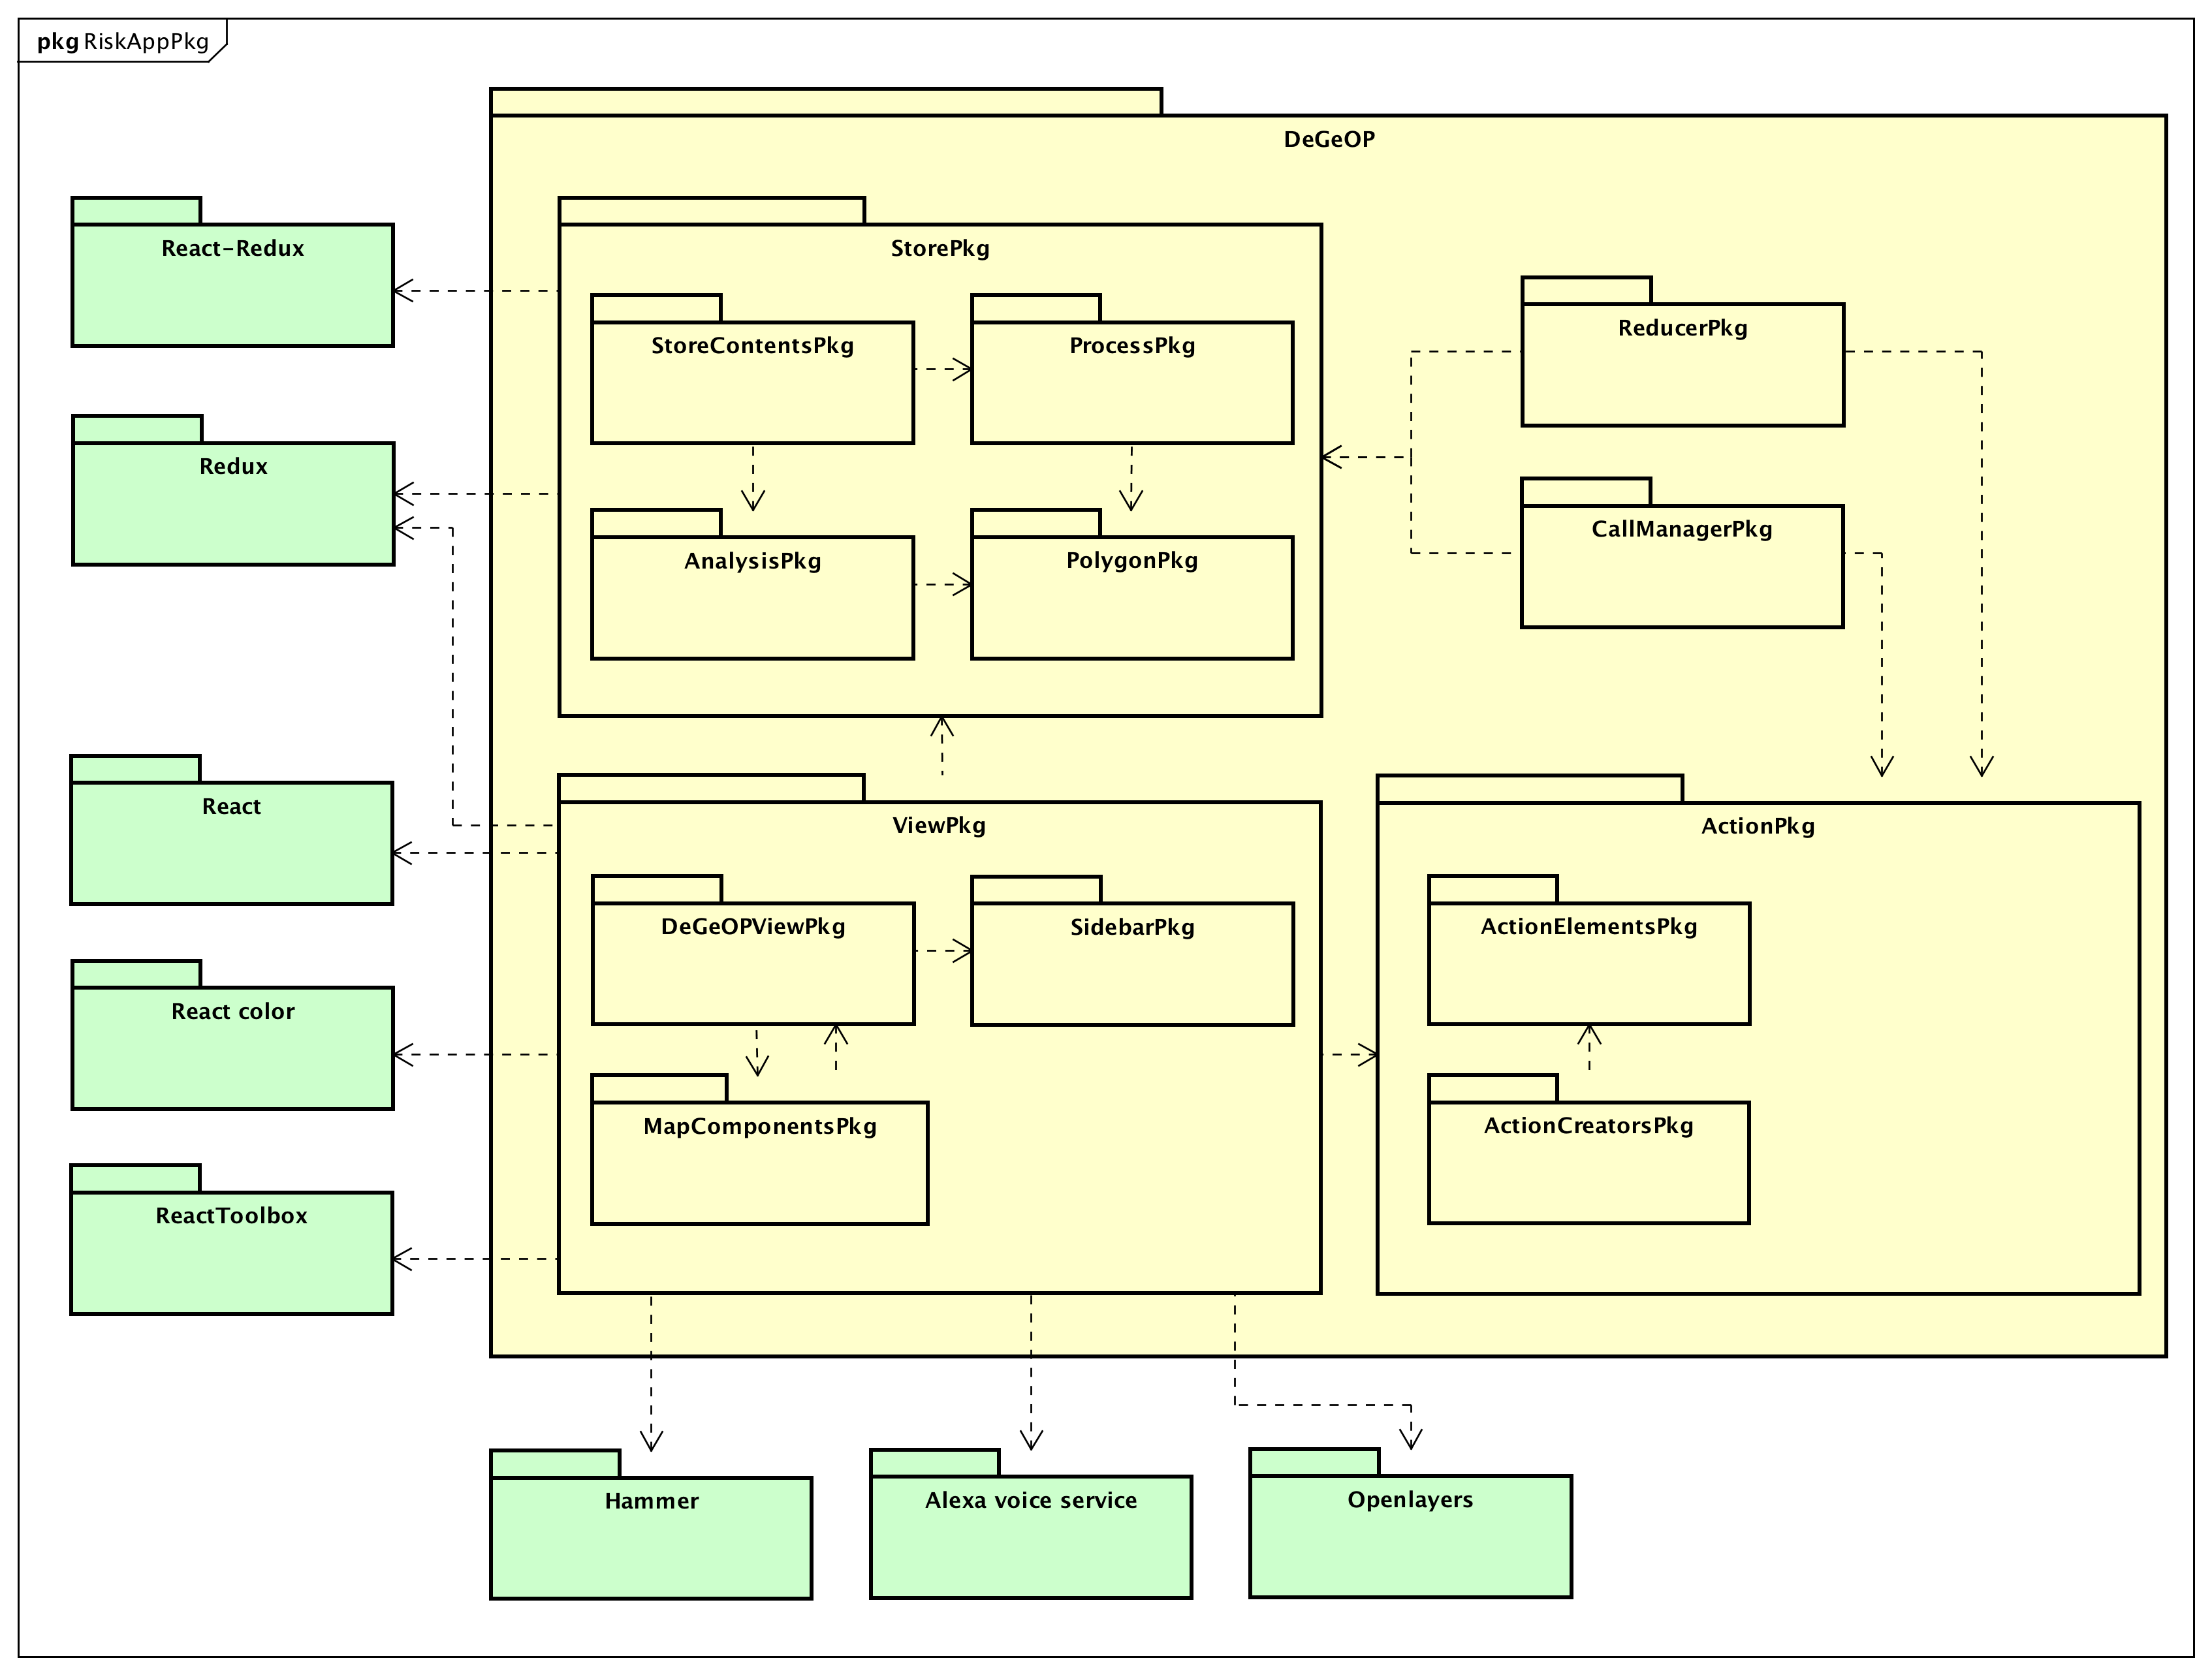
\includegraphics[width=\textwidth]{img/PkgDiagram/STDeGeOPPkg.png}
	\caption{Schema componente DeGeOP}
\end{figure}
\subsubsection{Informazioni sul package}
\begin{itemize}
	\item \textbf{descrizione:} racchiude tutte le componenti necessarie per il front-end del prodotto;
	\item \textbf{package contenuti:}
	\begin{itemize}
		\item DeGeOP::\hyperref[pkg::ActionPkg]{ActionPkg};
		\item DeGeOP::\hyperref[pkg::CallManagerPkg]{CallManagerPkg};
		\item DeGeOP::\hyperref[pkg::ReducerPkg]{ReducerPkg};
		\item DeGeOP::\hyperref[pkg::StorePkg]{StorePkg};
		\item DeGeOP::\hyperref[pkg::ViewPkg]{ViewPkg}.
	\end{itemize}
\end{itemize}
\newpage
\subsection{DeGeOP::StorePkg}
\label{pkg::StorePkg}
\begin{figure}[H]
	\centering
	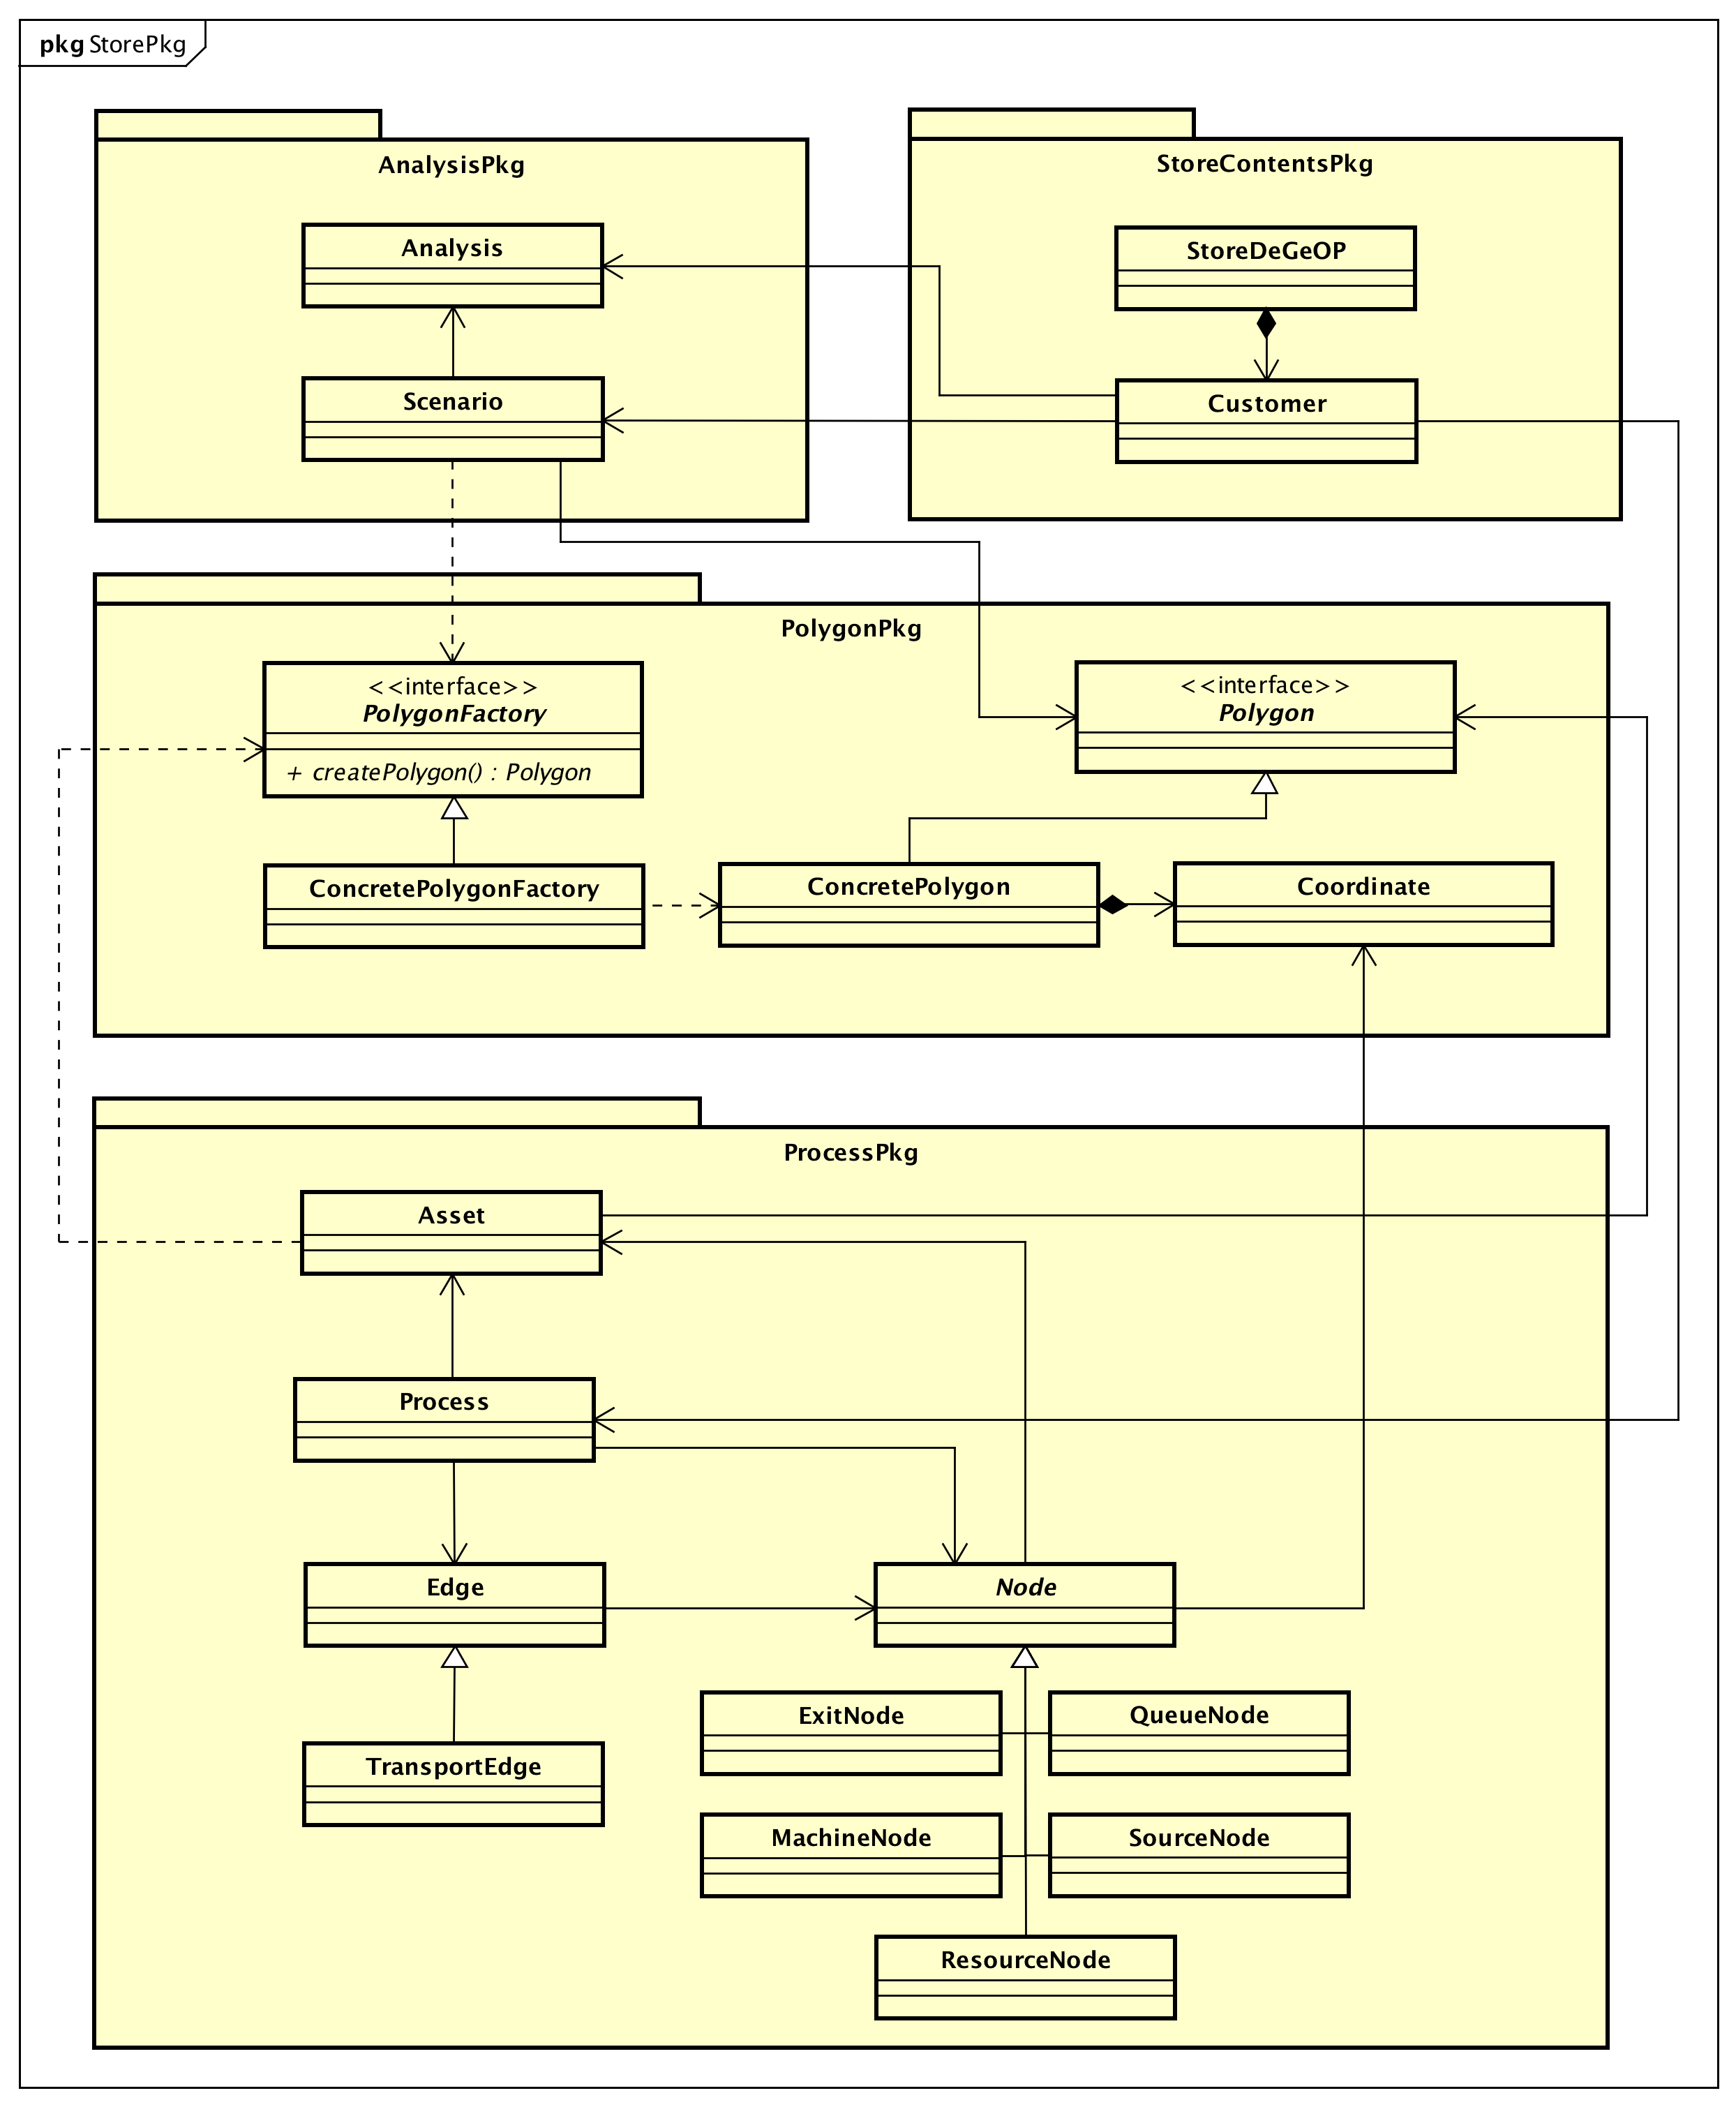
\includegraphics[width=\textwidth]{img/PkgDiagram/STStorePkg.png}
	\caption{Schema componente DeGeOP::StorePkg}
\end{figure}
\subsubsection{Informazioni sul package}
\begin{itemize}
	\item \textbf{descrizione:} racchiude le componenti utilizzate per la memorizzazione e rappresentazione dei dati;
	\item \textbf{padre:} \hyperref[pkg::DeGeOP]{DeGeOP};
	\item \textbf{package contenuti:}
	\begin{itemize}
		\item StorePkg::\hyperref[pkg::AnalysisPkg]{AnalysisPkg};
		\item StorePkg::\hyperref[pkg::PolygonPkg]{PolygonPkg};
		\item StorePkg::\hyperref[pkg::ProcessPkg]{ProcessPkg};
		\item StorePkg::\hyperref[pkg::StoreContentsPkg]{StoreContentsPkg}.
	\end{itemize}
	\item \textbf{interazioni con altri package:} 
	\begin{itemize}
		\item IN CallManagerPkg: subscribe sullo store;
		\item IN ReducerPkg: applicazione di cambiamenti di stato;
		\item IN ViewPkg: subscribe sullo store;
		\item OUT React-Redux: utilizzo di Provider per evitare di passare lo store come proprietà alle componenti React;
		\item OUT Redux: creazione Store utilizzando il metodo createStore().
	\end{itemize}
\end{itemize}
\newpage
\subsection{DeGeOP::StorePkg::StoreContentsPkg}
\label{pkg::StoreContentsPkg}
\subsubsection{Informazioni sul package}
\begin{itemize}
	\item \textbf{descrizione:} racchiude le componenti che implementano il concetto di store dell'architettura Redux;
	\item \textbf{padre:} \hyperref[pkg::StorePkg]{StorePkg};
	\item \textbf{interazioni con altri package:} 
	\begin{itemize}
		\item OUT AnalysisPkg: riferimento ad analisi di danno;
		\item OUT ProcessPkg: riferimento a processo;
		\item OUT React-Redux: utilizzo del Provider;
		\item OUT Redux: creazione store.
	\end{itemize}
	\item \textbf{classi contenute:}
	\begin{itemize}
		\item Customer;
		\item Options;
		\item StoreDeGeOP.
	\end{itemize}
\end{itemize}
\subsubsection{Classi}
\paragraph{Customer}
\begin{itemize}
	\item \textbf{descrizione:} rappresenta l'assicurando;
	\item \textbf{utilizzo:} viene utilizzato nello Store per memorizzare l'assicurando;
	\item \textbf{relazioni con altre classi:} 
	\begin{itemize}
		\item OUT Analysis;
		\item OUT Scenario.
	\end{itemize}
\end{itemize}
\paragraph{Options}
\begin{itemize}
	\item \textbf{descrizione:} classe contenente le associazioni tra codice e valore dei campi dati degli altri elementi dello store;
	\item \textbf{utilizzo:} viene utilizzata per associare codice e valore dei campi dati degli altri elementi dello store.
\end{itemize}
\paragraph{StoreDeGeOP}
\begin{itemize}
	\item \textbf{descrizione:} rappresenta una classe che incapsula uno Store creato utilizzando Redux;
	\item \textbf{utilizzo:} viene utilizzato per memorizzare lo stato dell'applicazione.
	Le componenti che effettuano il subscribe sullo Store verranno notificate ad ogni cambiamento di stato dello Store.
\end{itemize}
\newpage
\subsection{DeGeOP::StorePkg::ProcessPkg}
\label{pkg::ProcessPkg}
\subsubsection{Informazioni sul package}
\begin{itemize}
	\item \textbf{descrizione:} racchiude le componenti necessarie alla rappresentazione del processo produttivo dell'assicurando;
	\item \textbf{padre:} \hyperref[pkg::StorePkg]{StorePkg};
	\item \textbf{interazioni con altri package:} 
	\begin{itemize}
		\item IN StoreContentsPkg: riferimento a processo;
		\item OUT PolygonPkg: riferimento ad un poligono.
	\end{itemize}
	\item \textbf{classi contenute:}
	\begin{itemize}
		\item Asset;
		\item Edge;
		\item ExitNode;
		\item MachineNode;
		\item Node;
		\item Process;
		\item QueueNode;
		\item ResourceNode;
		\item SourceNode;
		\item TransportEdge.
	\end{itemize}
\end{itemize}
\subsubsection{Classi}
\paragraph{Asset}
\begin{itemize}
	\item \textbf{descrizione:} rappresenta un fabbricato di interesse per il processo produttivo dell'assicurando;
	\item \textbf{utilizzo:} sono contenuti all'interno di Process.
\end{itemize}
\paragraph{Edge}
\begin{itemize}
	\item \textbf{descrizione:} rappresenta un arco che collega due nodi tra di loro; un arco indica che i nodi sono in correlazione tra di loro;
	\item \textbf{utilizzo:} è contenuto all'interno di Process.
\end{itemize}
\paragraph{ExitNode}
\begin{itemize}
	\item \textbf{descrizione:} rappresenta un nodo di tipo Uscita;
	\item \textbf{utilizzo:} è contenuto all'interno di Process.
\end{itemize}
\paragraph{MachineNode}
\begin{itemize}
	\item \textbf{descrizione:} rappresenta un nodo di tipo Macchina;
	\item \textbf{utilizzo:} è contenuto all'interno di Process.
\end{itemize}
\paragraph{Node}
\begin{itemize}
	\item \textbf{descrizione:} rappresenta un nodo contenuto all'interno di un Asset ;
	\item \textbf{utilizzo:} è contenuto all'interno di Process.
\end{itemize}
\paragraph{Process}
\begin{itemize}
	\item \textbf{descrizione:} rappresenta un processo produttivo dell'azienda dell'assicurando;
	\item \textbf{utilizzo:} è memorizzato nello Store.
\end{itemize}
\paragraph{QueueNode}
\begin{itemize}
	\item \textbf{descrizione:} rappresenta un nodo di tipo Coda;
	\item \textbf{utilizzo:} è contenuto all'interno di Process.
\end{itemize}
\paragraph{ResourceNode}
\begin{itemize}
	\item \textbf{descrizione:} rappresenta un nodo di tipo Risorsa;
	\item \textbf{utilizzo:} è contenuto all'interno di Process.
\end{itemize}
\paragraph{SourceNode}
\begin{itemize}
	\item \textbf{descrizione:} rappresenta un nodo di tipo Sorgente;
	\item \textbf{utilizzo:} è contenuto all'interno di Process.
\end{itemize}
\paragraph{TransportEdge}
\begin{itemize}
	\item \textbf{descrizione:} rappresenta un arco di tipo Trasporto;
	\item \textbf{utilizzo:} è contenuto all'interno di Process.
\end{itemize}
\newpage
\subsection{DeGeOP::StorePkg::AnalysisPkg}
\label{pkg::AnalysisPkg}
\subsubsection{Informazioni sul package}
\begin{itemize}
	\item \textbf{descrizione:} racchiude le componenti necessarie alla rappresentazione dell'analisi di danno relative al processo produttivo dell'assicurando;
	\item \textbf{padre:} \hyperref[pkg::StorePkg]{StorePkg};
	\item \textbf{interazioni con altri package:} 
	\begin{itemize}
		\item IN StoreContentsPkg: riferimento ad analisi di danno;
		\item OUT PolygonPkg: riferimento ad un poligono.
	\end{itemize}
	\item \textbf{classi contenute:}
	\begin{itemize}
		\item Analysis;
		\item Scenario.
	\end{itemize}
\end{itemize}
\subsubsection{Classi}
\paragraph{Analysis}
\begin{itemize}
	\item \textbf{descrizione:} rappresenta un risultato di un'analisi di danno relativo ad uno scenario;
	\item \textbf{utilizzo:} i metodi di questa classe saranno utilizzati per calcolare dati riassuntivi sull'analisi di danno;
	\item \textbf{relazioni con altre classi:} 
	\begin{itemize}
		\item IN Customer.
	\end{itemize}
\end{itemize}
\paragraph{Scenario}
\begin{itemize}
	\item \textbf{descrizione:} rappresenta uno scenario di danno;
	\item \textbf{utilizzo:} viene utilizzata nello store per rappresentare gli scenari di danno;
	\item \textbf{relazioni con altre classi:} 
	\begin{itemize}
		\item IN Customer.
	\end{itemize}
\end{itemize}
\newpage
\subsection{DeGeOP::StorePkg::PolygonPkg}
\label{pkg::PolygonPkg}
\subsubsection{Informazioni sul package}
\begin{itemize}
	\item \textbf{descrizione:} racchiude le componenti necessarie alla rappresentazione dell'area degli asset e degli scenari di danno;
	\item \textbf{padre:} \hyperref[pkg::StorePkg]{StorePkg};
	\item \textbf{interazioni con altri package:} 
	\begin{itemize}
		\item IN AnalysisPkg: riferimento ad un poligono;
		\item IN ProcessPkg: riferimento ad un poligono.
	\end{itemize}
	\item \textbf{classi contenute:}
	\begin{itemize}
		\item ConcretePolygon;
		\item ConcretePolygonFactory;
		\item Coordinate;
		\item Polygon;
		\item PolygonFactory.
	\end{itemize}
\end{itemize}
\subsubsection{Classi}
\paragraph{ConcretePolygon}
\begin{itemize}
	\item \textbf{descrizione:} rappresenta un poligono;
	\item \textbf{utilizzo:} viene istanziata da ConcretePolygonFactory; viene utilizzata in Asset e Scenario.
\end{itemize}
\paragraph{ConcretePolygonFactory}
\begin{itemize}
	\item \textbf{descrizione:} gestisce la creazione concreta dei poligoni;
	\item \textbf{utilizzo:} implementazione di PolygonFactory; è la classe concreta da istanziare per gestire la creazione di un poligono.
\end{itemize}
\paragraph{Coordinate}
\begin{itemize}
	\item \textbf{descrizione:} rappresenta una coordinata geografica;
	\item \textbf{utilizzo:} è utilizzata all'interno di Polygon per delimitarne i suoi vertici.
\end{itemize}
\paragraph{Polygon}
\begin{itemize}
	\item \textbf{descrizione:} interfaccia che rappresenta il poligono;
	\item \textbf{utilizzo:} fornisce i metodi del poligono.
\end{itemize}
\paragraph{PolygonFactory}
\begin{itemize}
	\item \textbf{descrizione:} interfaccia che si occupa della costruzione dei poligoni;
	\item \textbf{utilizzo:} viene usata dalle classi Scenario e Asset per la costruzione dei poligoni.
\end{itemize}
\newpage
\subsection{DeGeOP::ReducerPkg}
\label{pkg::ReducerPkg}
\begin{figure}[H]
	\centering
	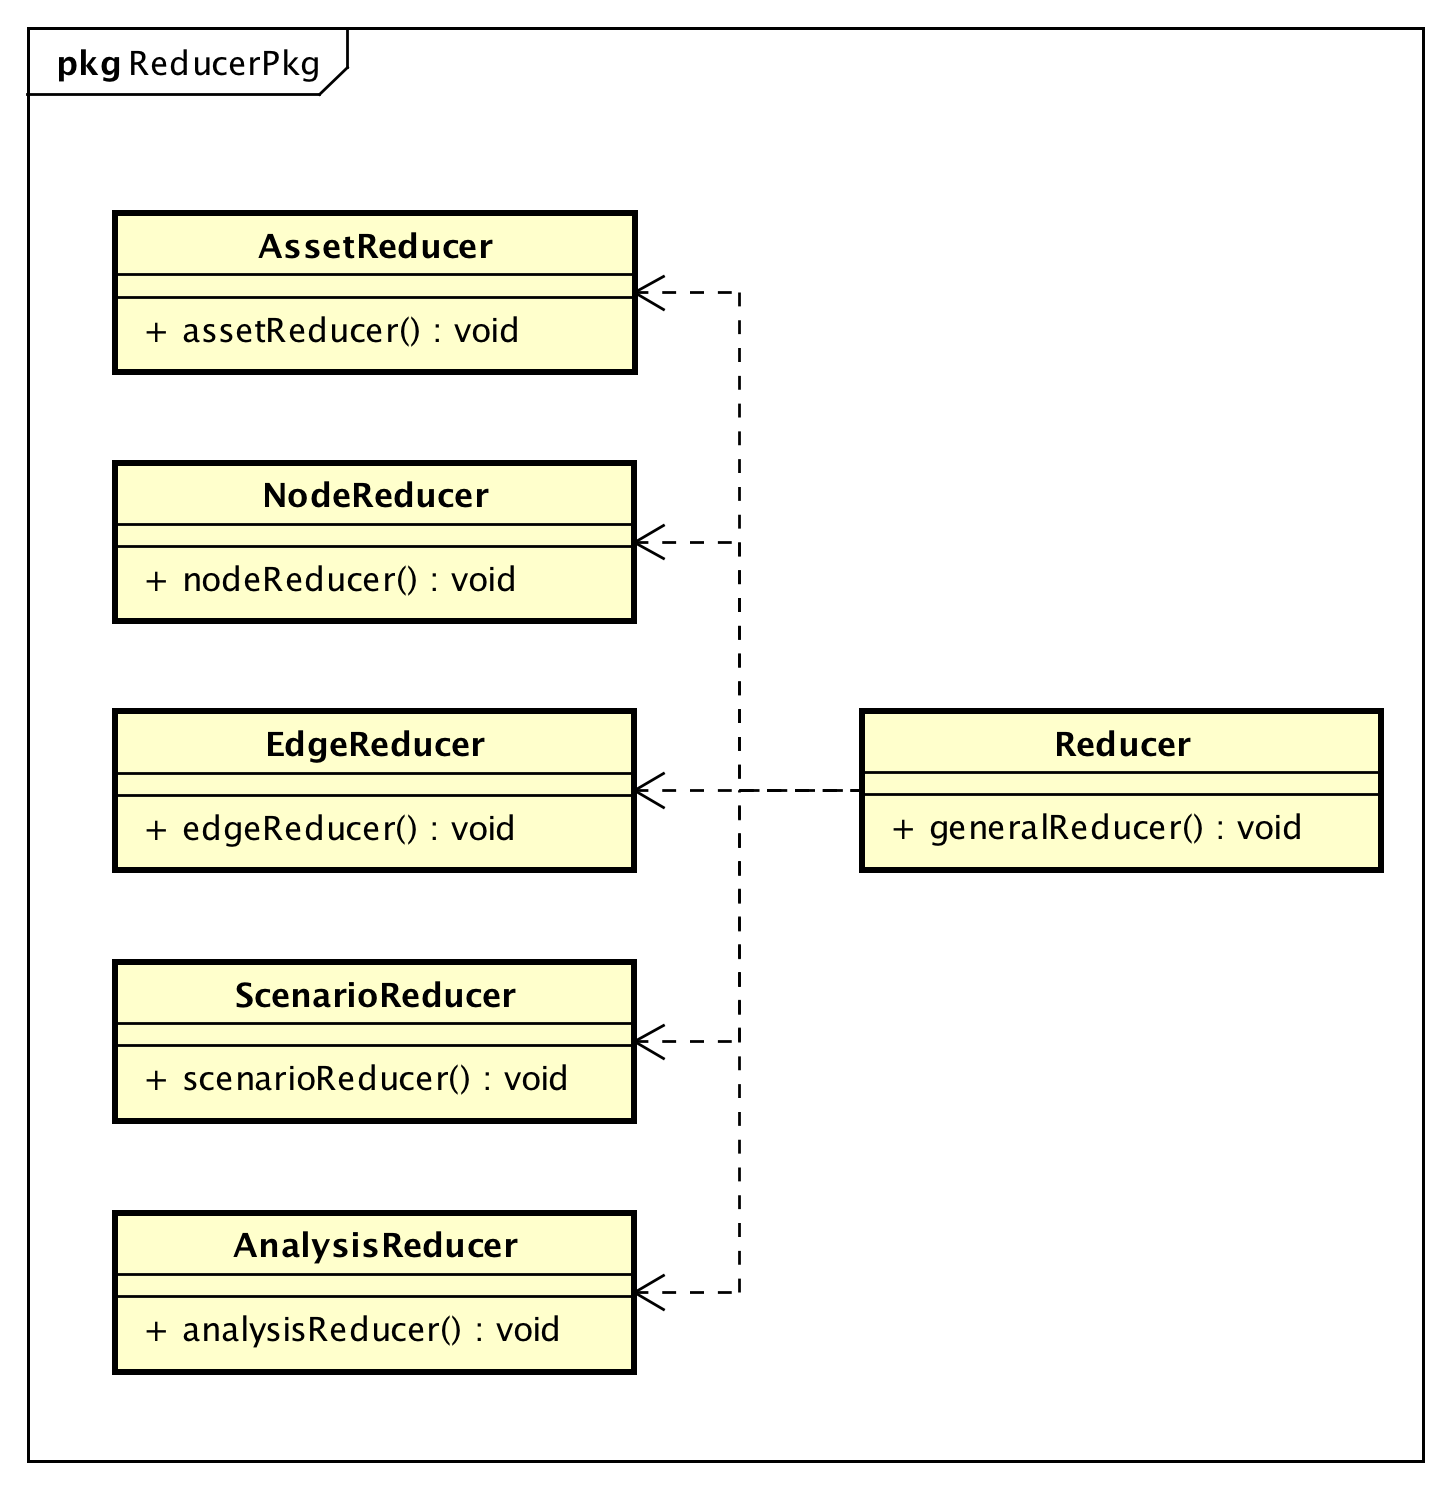
\includegraphics[width=\textwidth]{img/PkgDiagram/STReducerPkg.png}
	\caption{Schema componente DeGeOP::ReducerPkg}
\end{figure}
\subsubsection{Informazioni sul package}
\begin{itemize}
	\item \textbf{descrizione:} racchiude le componenti necessarie all'implementazione dei reducer secondo l'architettura Redux;
	\item \textbf{padre:} \hyperref[pkg::DeGeOP]{DeGeOP};
	\item \textbf{interazioni con altri package:} 
	\begin{itemize}
		\item OUT ActionPkg: utilizzo di azioni ;
		\item OUT StorePkg: applicazione di cambiamenti di stato.
	\end{itemize}
	\item \textbf{classi contenute:}
	\begin{itemize}
		\item AnalysisReducer;
		\item AssetReducer;
		\item EdgeReducer;
		\item NodeReducer;
		\item OptionReducer;
		\item Reducer;
		\item ScenarioReducer.
	\end{itemize}
\end{itemize}
\subsubsection{Classi}
\paragraph{AnalysisReducer}
\begin{itemize}
	\item \textbf{descrizione:} rappresenta il reducer dell'analisi;
	\item \textbf{utilizzo:} il suo metodo gestisce le operazioni sullo store riguardanti le analisi;
	\item \textbf{relazioni con altre classi:} 
	\begin{itemize}
		\item IN Reducer.
	\end{itemize}
\end{itemize}
\paragraph{AssetReducer}
\begin{itemize}
	\item \textbf{descrizione:} rappresenta il reducer dell'asset;
	\item \textbf{utilizzo:} il suo metodo gestisce le operazioni sullo store riguardanti l'asset.
\end{itemize}
\paragraph{EdgeReducer}
\begin{itemize}
	\item \textbf{descrizione:} rappresenta il reducer dell'arco;
	\item \textbf{utilizzo:} il suo metodo gestisce le operazioni sullo store riguardanti gli archi.
\end{itemize}
\paragraph{NodeReducer}
\begin{itemize}
	\item \textbf{descrizione:} rappresenta il reducer del nodo;
	\item \textbf{utilizzo:} il suo metodo gestisce le operazioni sullo store riguardanti i nodi.
\end{itemize}
\paragraph{OptionReducer}
\begin{itemize}
	\item \textbf{descrizione:} rappresenta il reducer delle option;
	\item \textbf{utilizzo:} il suo metodo gestisce le operazioni sullo store riguardanti l'asset.
\end{itemize}
\paragraph{Reducer}
\begin{itemize}
	\item \textbf{descrizione:} accetta una action generica in input e la reindirizza al giusto reducer;
	\item \textbf{utilizzo:} il suo metodo viene utilizzato per catturare un'azione e generare un nuovo stato sullo Store;
	\item \textbf{relazioni con altre classi:} 
	\begin{itemize}
		\item OUT AnalysisReducer;
		\item OUT ScenarioReducer.
	\end{itemize}
\end{itemize}
\paragraph{ScenarioReducer}
\begin{itemize}
	\item \textbf{descrizione:} rappresenta il reducer dello scenario;
	\item \textbf{utilizzo:} il suo metodo gestisce le operazioni sullo store riguardanti gli scenari;
	\item \textbf{relazioni con altre classi:} 
	\begin{itemize}
		\item IN Reducer.
	\end{itemize}
\end{itemize}
\newpage
\subsection{DeGeOP::CallManagerPkg}
\label{pkg::CallManagerPkg}
\begin{figure}[H]
	\centering
	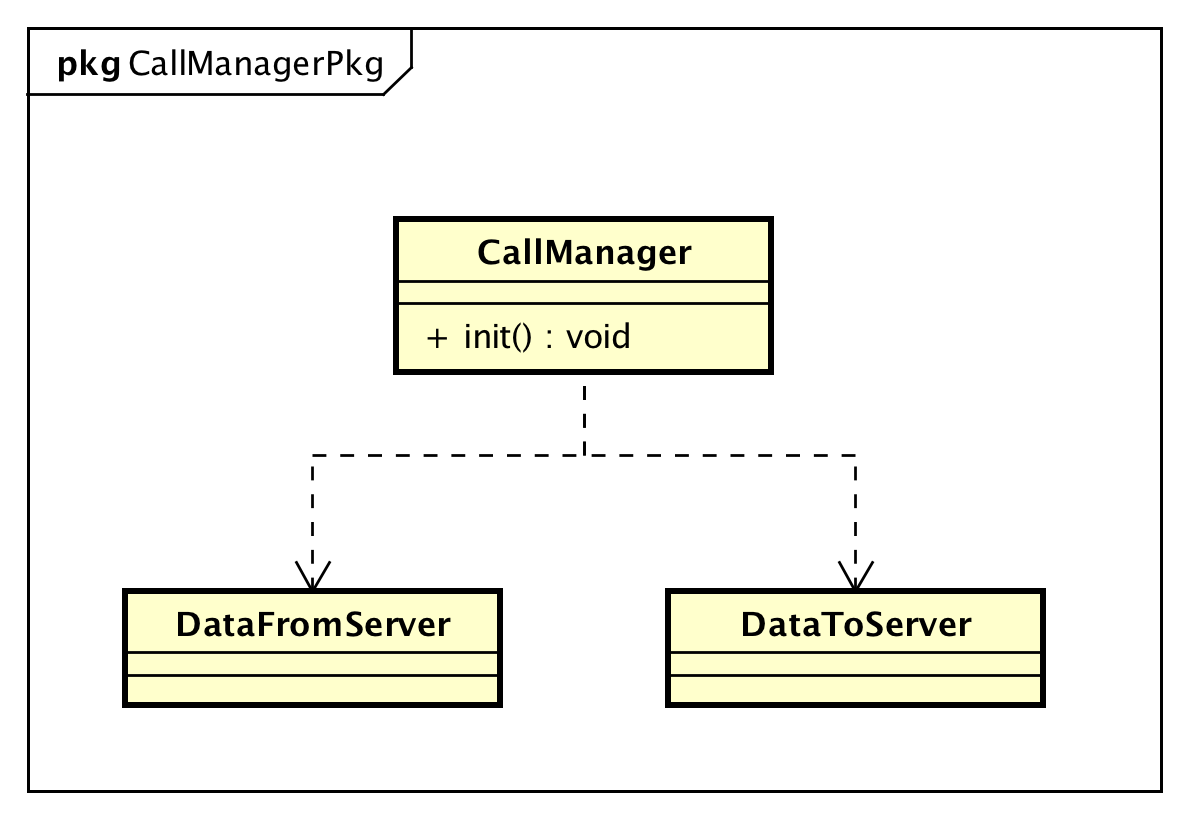
\includegraphics[width=\textwidth]{img/PkgDiagram/STCallManagerPkg.png}
	\caption{Schema componente DeGeOP::CallManagerPkg}
\end{figure}
\subsubsection{Informazioni sul package}
\begin{itemize}
	\item \textbf{descrizione:} racchiude le componenti necessarie alla comunicazione dei dati verso il server;
	\item \textbf{padre:} \hyperref[pkg::DeGeOP]{DeGeOP};
	\item \textbf{interazioni con altri package:} 
	\begin{itemize}
		\item OUT ActionPkg: dispatch di azioni;
		\item OUT StorePkg: subscribe sullo store.
	\end{itemize}
	\item \textbf{classi contenute:}
	\begin{itemize}
		\item CallManager;
		\item DataFromServer;
		\item DataToServer.
	\end{itemize}
\end{itemize}
\subsubsection{Classi}
\paragraph{CallManager}
\begin{itemize}
	\item \textbf{descrizione:} rappresenta il gestore delle chiamate da e verso il server;
	\item \textbf{utilizzo:} viene usato per effettuare chiamate REST da e verso il server. I suoi metodi si occupano di inizializzare lo Store emettendo Action quando l'applicazione viene aperta. Sfrutta i metodi della classe DataFromServer per effettuare la conversione da JSON ad oggetto logico. Inoltre, la classe effettuerà il subscribe allo Store per ricevere i cambiamenti di stato e mantenere aggiornate le informazioni sul server. La classe avrà un metodo che identifica cos'è cambiato nello Store e farà la chiamata REST appropriata, sfruttando la classe DataToServer per trasformare l'oggetto logico in JSON.
\end{itemize}
\paragraph{DataFromServer}
\begin{itemize}
	\item \textbf{descrizione:} rappresenta il gestore dei dati ricevuti dal server;
	\item \textbf{utilizzo:} gestisce i dati ricevuti dal server. I suoi metodi si occupano di effettuare la conversione dei JSON ricevuti dal server in oggetti logici.
\end{itemize}
\paragraph{DataToServer}
\begin{itemize}
	\item \textbf{descrizione:} rappresenta il gestore dei dati da inviare verso il server;
	\item \textbf{utilizzo:} gestisce i dati che dovranno essere inviati al server. I suoi metodi effettuano la conversione degli oggetti logici in JSON.
\end{itemize}
\newpage
\subsection{DeGeOP::ActionPkg}
\label{pkg::ActionPkg}
\begin{figure}[H]
	\centering
	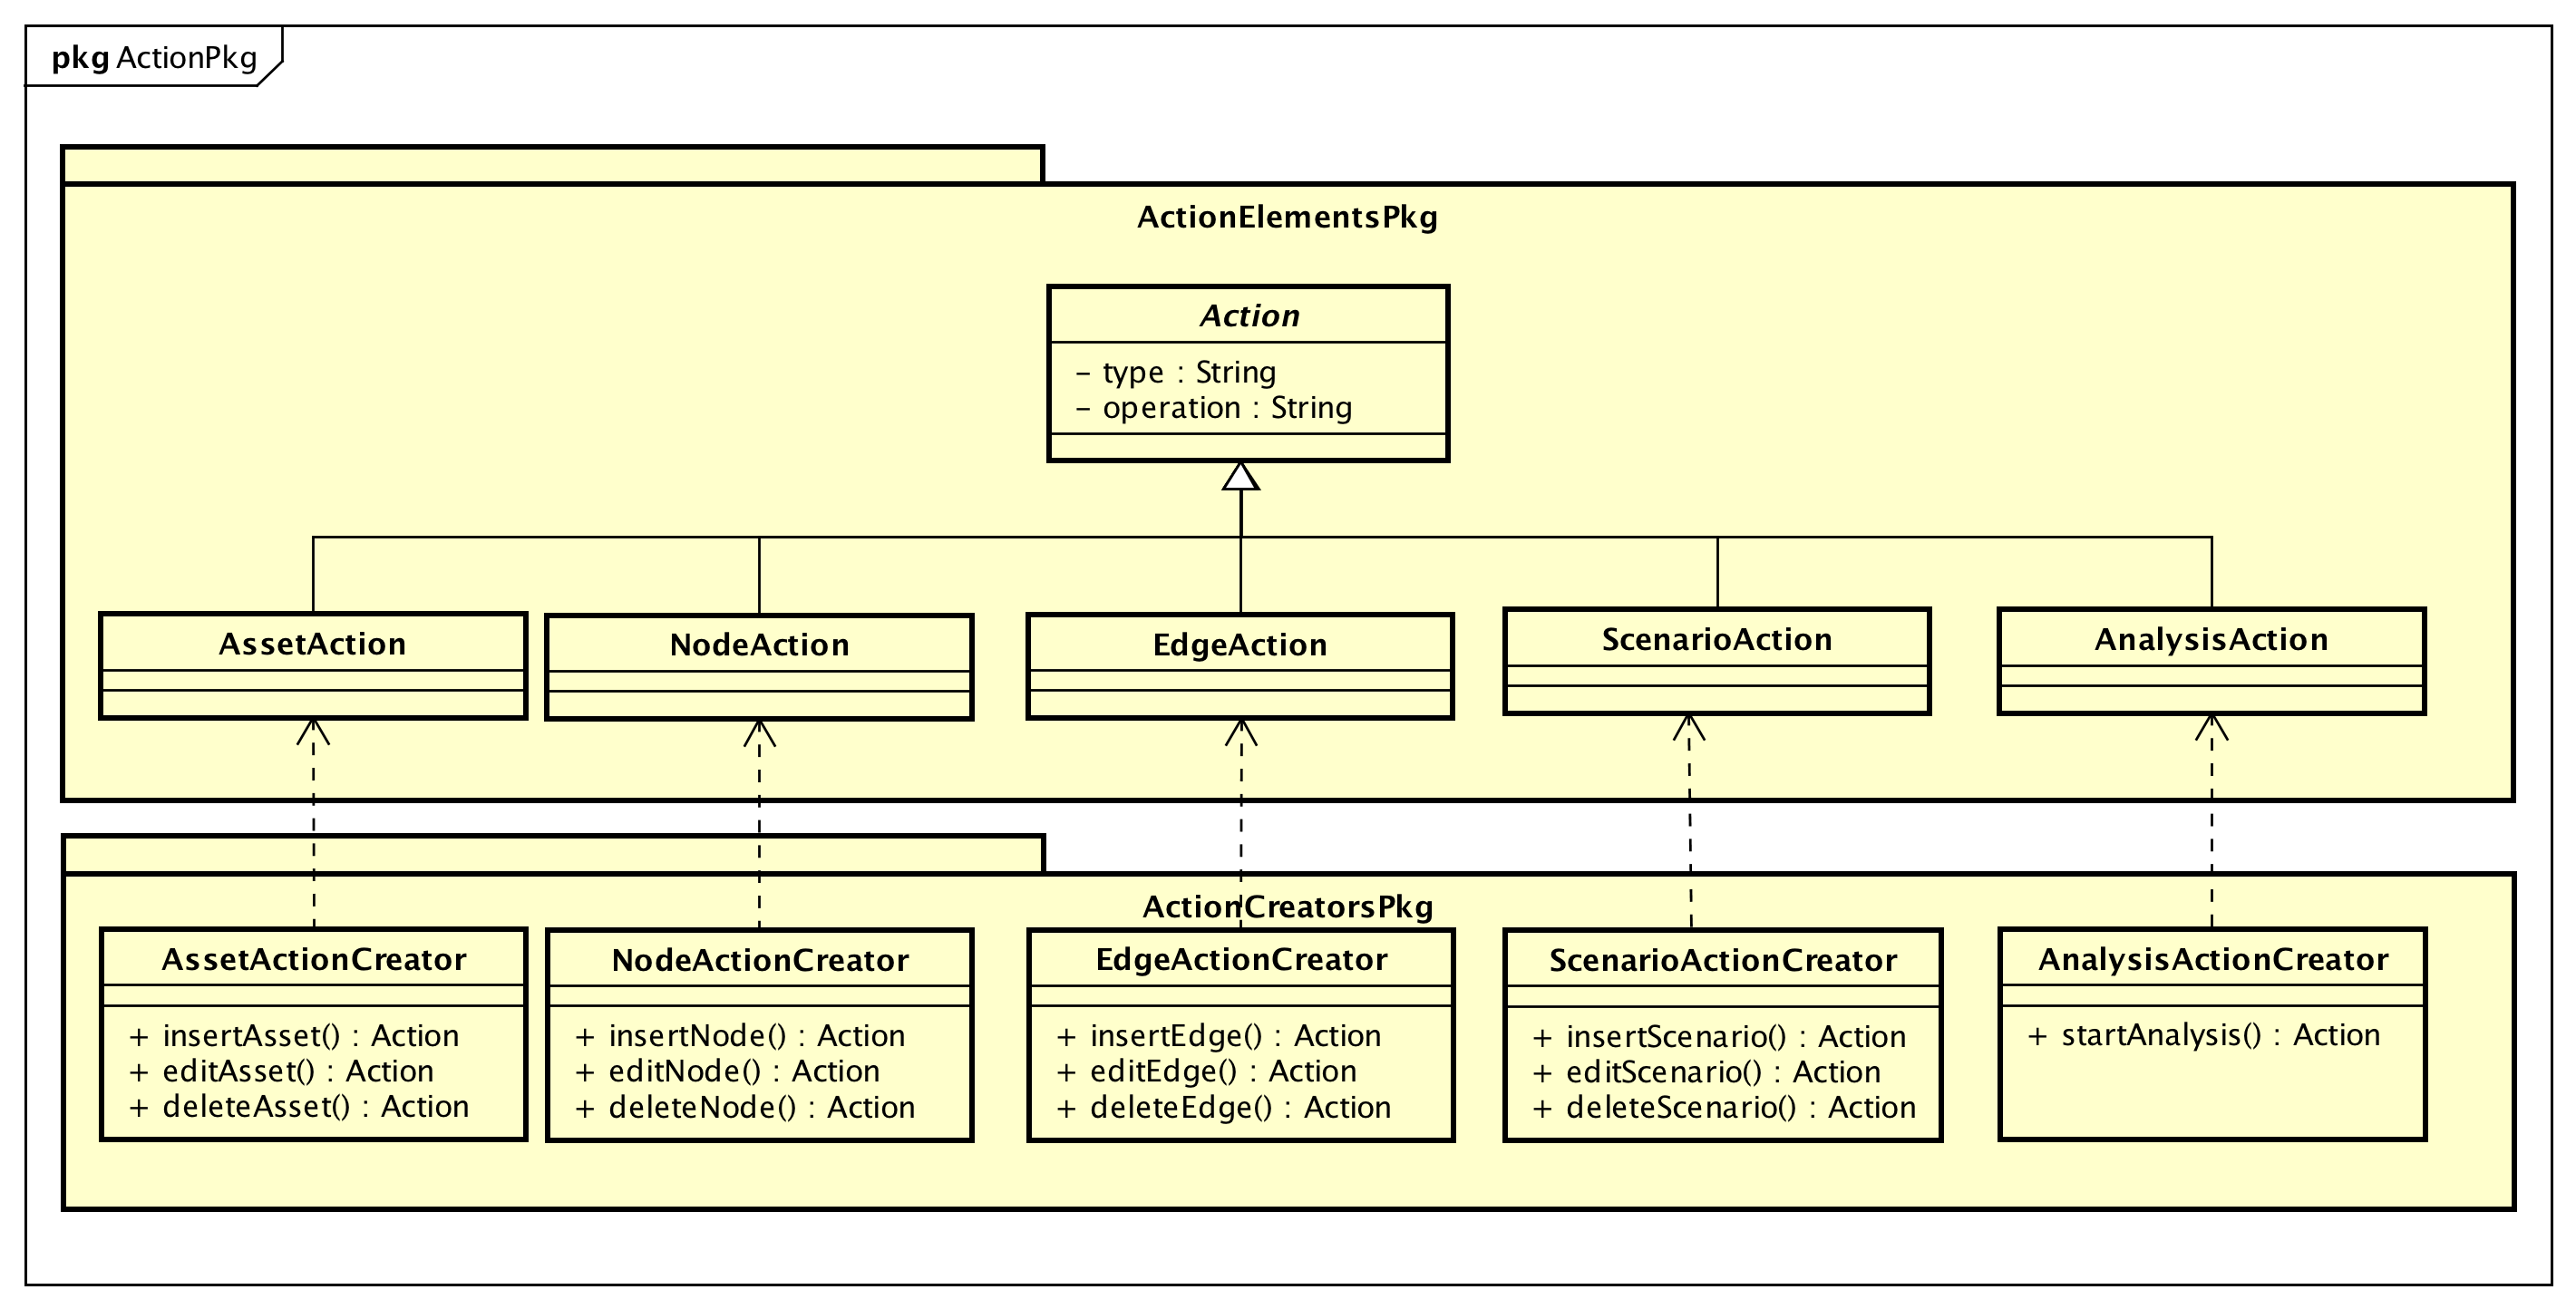
\includegraphics[width=\textwidth]{img/PkgDiagram/STActionPkg.png}
	\caption{Schema componente DeGeOP::ActionPkg}
\end{figure}
\subsubsection{Informazioni sul package}
\begin{itemize}
	\item \textbf{descrizione:} racchiude le componenti utilizzate per implementare le action dell'architettura Redux. Le action vengono create e ne viene fatto il dispatch verso lo store. Un reducer gestirà una action per produrre un cambiamento di stato sullo store;
	\item \textbf{padre:} \hyperref[pkg::DeGeOP]{DeGeOP};
	\item \textbf{package contenuti:}
	\begin{itemize}
		\item ActionPkg::\hyperref[pkg::ActionCreatorsPkg]{ActionCreatorsPkg};
		\item ActionPkg::\hyperref[pkg::ActionElementsPkg]{ActionElementsPkg}.
	\end{itemize}
	\item \textbf{interazioni con altri package:} 
	\begin{itemize}
		\item IN CallManagerPkg: dispatch di azioni;
		\item IN ReducerPkg: utilizzo di azioni ;
		\item IN ViewPkg: dispatch di azioni.
	\end{itemize}
	\item \textbf{classi contenute:}
	\begin{itemize}
		\item EdgeAction.
	\end{itemize}
\end{itemize}
\subsubsection{Classi}
\paragraph{EdgeAction}
\begin{itemize}
	\item \textbf{descrizione:} rappresenta un'azione relativa agli archi;
	\item \textbf{utilizzo:} l'azione viene creata da un apposito ActionCreator per essere poi inviata ad un reducer.
\end{itemize}
\newpage
\subsection{DeGeOP::ActionPkg::ActionElementsPkg}
\label{pkg::ActionElementsPkg}
\subsubsection{Informazioni sul package}
\begin{itemize}
	\item \textbf{descrizione:} racchiude le componenti che rappresentano effettivamente le azioni;
	\item \textbf{padre:} \hyperref[pkg::ActionPkg]{ActionPkg};
	\item \textbf{interazioni con altri package:} 
	\begin{itemize}
		\item IN ActionCreatorsPkg: creazione di azioni.
	\end{itemize}
	\item \textbf{classi contenute:}
	\begin{itemize}
		\item Action;
		\item AnalysisAction;
		\item AssetAction;
		\item NodeAction;
		\item OptionAction;
		\item ScenarioAction.
	\end{itemize}
\end{itemize}
\subsubsection{Classi}
\paragraph{Action}
\begin{itemize}
	\item \textbf{descrizione:} una classe astratta che rappresenta una generica azione di cui può essere fatto il dispatch;
	\item \textbf{utilizzo:} i suoi membri vengono usati dai reducer per completare una azione.
\end{itemize}
\paragraph{AnalysisAction}
\begin{itemize}
	\item \textbf{descrizione:} rappresenta un'azione relativa alle analisi di danno;
	\item \textbf{utilizzo:} l'azione viene creata da un apposito ActionCreator per essere poi inviata ad un reducer;
	\item \textbf{relazioni con altre classi:} 
	\begin{itemize}
		\item IN AnalysisActionCreator.
	\end{itemize}
\end{itemize}
\paragraph{AssetAction}
\begin{itemize}
	\item \textbf{descrizione:} rappresenta un'azione relativa agli asset;
	\item \textbf{utilizzo:} l'azione viene creata da un apposito ActionCreator per essere poi inviata ad un reducer.
\end{itemize}
\paragraph{NodeAction}
\begin{itemize}
	\item \textbf{descrizione:} rappresenta un'azione relativa ai nodi;
	\item \textbf{utilizzo:} l'azione viene creata da un apposito ActionCreator per essere poi inviata ad un reducer.
\end{itemize}
\paragraph{OptionAction}
\begin{itemize}
	\item \textbf{descrizione:} rappresenta un'azione relativa all'oggetto option;
	\item \textbf{utilizzo:} l'azione viene creata da un apposito ActionCreator per essere poi inviata ad un reducer.
\end{itemize}
\paragraph{ScenarioAction}
\begin{itemize}
	\item \textbf{descrizione:} rappresenta un'azione relativa agli scenari di danno;
	\item \textbf{utilizzo:} l'azione viene creata da un apposito ActionCreator per essere poi inviata ad un reducer;
	\item \textbf{relazioni con altre classi:} 
	\begin{itemize}
		\item IN ScenarioActionCreator.
	\end{itemize}
\end{itemize}
\newpage
\subsection{DeGeOP::ActionPkg::ActionCreatorsPkg}
\label{pkg::ActionCreatorsPkg}
\subsubsection{Informazioni sul package}
\begin{itemize}
	\item \textbf{descrizione:} racchiude le componenti che gestiscono la creazione delle azioni;
	\item \textbf{padre:} \hyperref[pkg::ActionPkg]{ActionPkg};
	\item \textbf{interazioni con altri package:} 
	\begin{itemize}
		\item OUT ActionElementsPkg: creazione di azioni.
	\end{itemize}
	\item \textbf{classi contenute:}
	\begin{itemize}
		\item AnalysisActionCreator;
		\item AssetActionCreator;
		\item EdgeActionCreator;
		\item NodeActionCreator;
		\item OptionActionCreator;
		\item ScenarioActionCreator.
	\end{itemize}
\end{itemize}
\subsubsection{Classi}
\paragraph{AnalysisActionCreator}
\begin{itemize}
	\item \textbf{descrizione:} rappresenta la factory di azioni relative alle analisi di danno;
	\item \textbf{utilizzo:} i suoi metodi sono chiamati dalla View e dal CallManager per la creazione di azioni relative alle analisi di danno;
	\item \textbf{relazioni con altre classi:} 
	\begin{itemize}
		\item OUT AnalysisAction.
	\end{itemize}
\end{itemize}
\paragraph{AssetActionCreator}
\begin{itemize}
	\item \textbf{descrizione:} rappresenta la factory di azioni relative agli asset;
	\item \textbf{utilizzo:} i suoi metodi sono chiamati dalla View e dal CallManager per la creazione di azioni relative agli asset.
\end{itemize}
\paragraph{EdgeActionCreator}
\begin{itemize}
	\item \textbf{descrizione:} rappresenta la factory di azioni relative agli archi;
	\item \textbf{utilizzo:} i suoi metodi sono chiamati dalla View e dal CallManager per la creazione di azioni relative agli archi.
\end{itemize}
\paragraph{NodeActionCreator}
\begin{itemize}
	\item \textbf{descrizione:} rappresenta la factory di azioni relative ai nodi;
	\item \textbf{utilizzo:} i suoi metodi sono chiamati dalla View e dal CallManager per la creazione di azioni relative ai nodi.
\end{itemize}
\paragraph{OptionActionCreator}
\begin{itemize}
	\item \textbf{descrizione:} rappresenta la factory di azioni relative agli asset;
	\item \textbf{utilizzo:} i suoi metodi sono chiamati dalla View e dal CallManager per la creazione di azioni relative agli asset.
\end{itemize}
\paragraph{ScenarioActionCreator}
\begin{itemize}
	\item \textbf{descrizione:} rappresenta la factory di azioni relative agli scenari di danno;
	\item \textbf{utilizzo:} i suoi metodi sono chiamati dalla View e dal CallManager per la creazione di azioni relative agli scenari di danno;
	\item \textbf{relazioni con altre classi:} 
	\begin{itemize}
		\item OUT ScenarioAction.
	\end{itemize}
\end{itemize}
\newpage
\subsection{DeGeOP::ViewPkg}
\label{pkg::ViewPkg}
\begin{figure}[H]
	\centering
	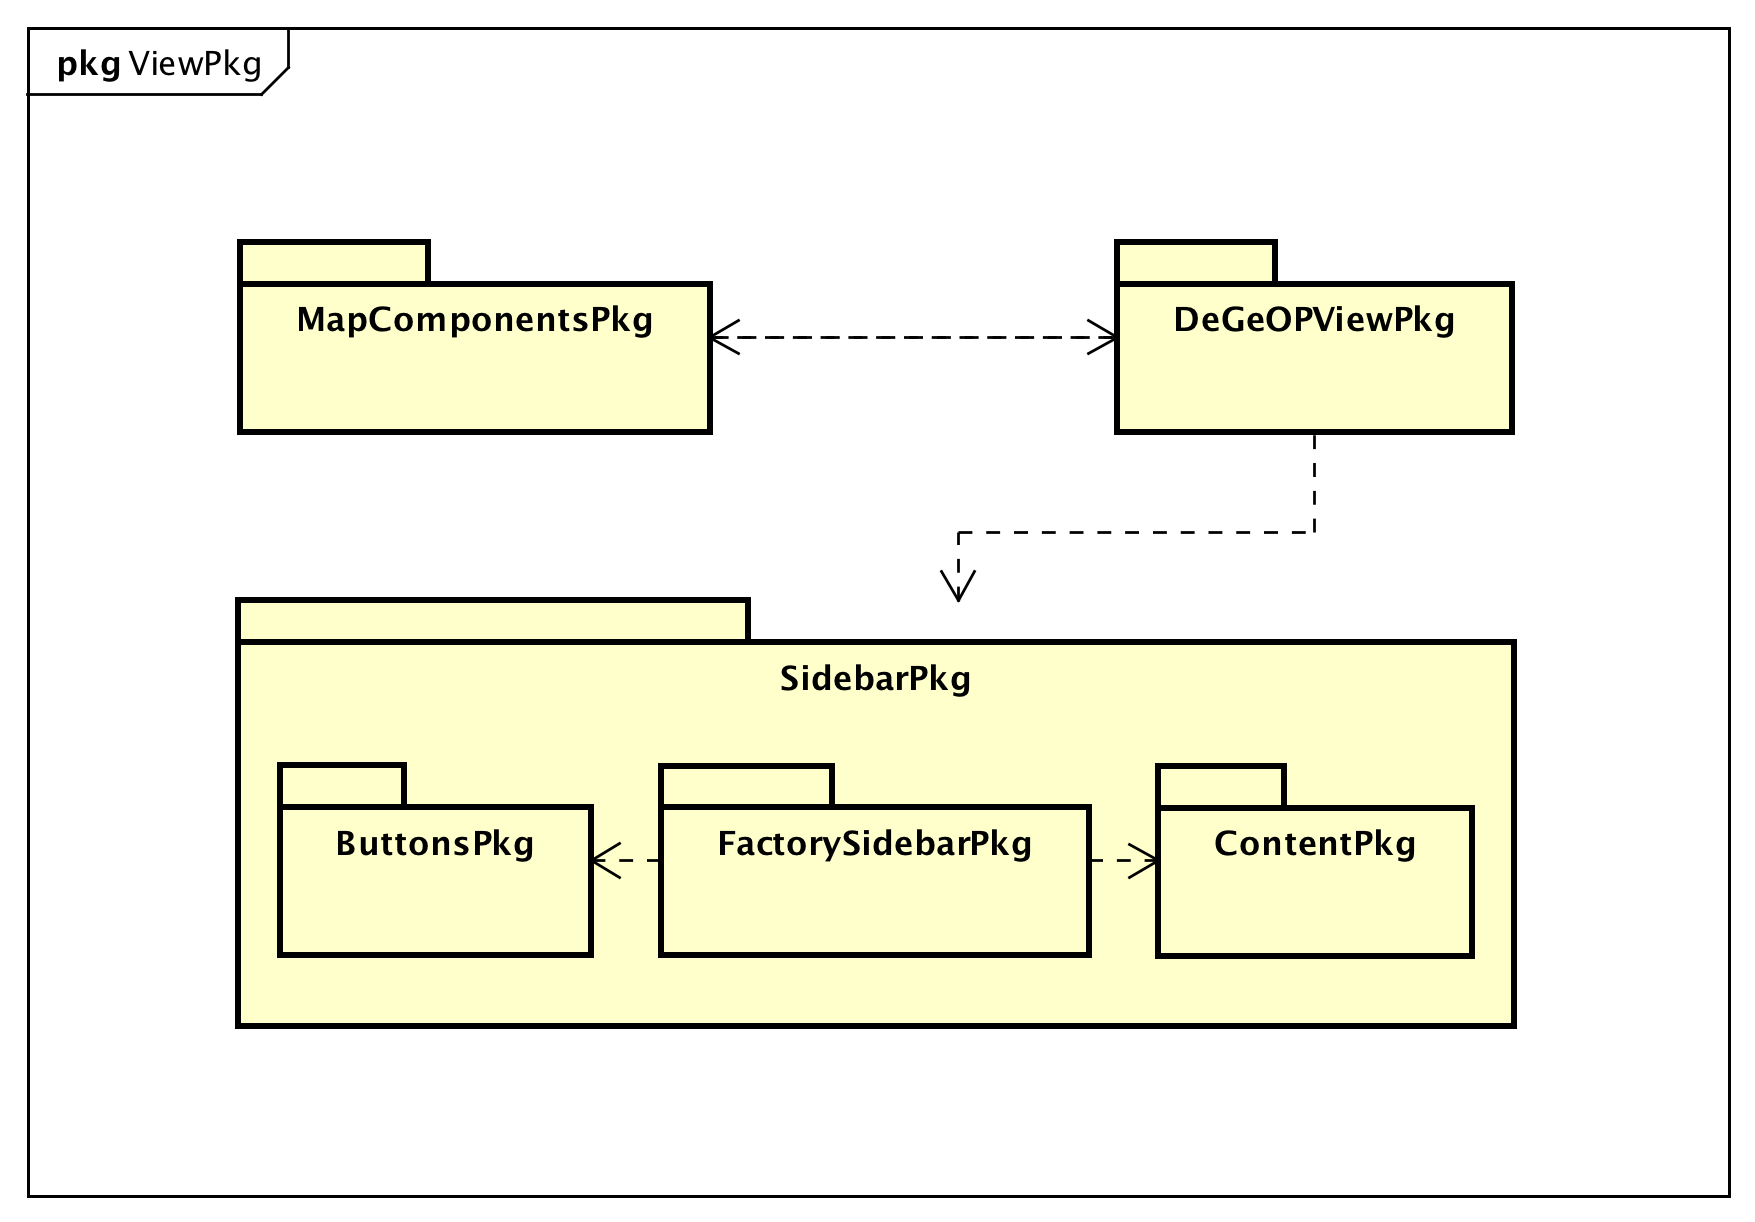
\includegraphics[width=\textwidth]{img/PkgDiagram/STViewPkg.png}
	\caption{Schema componente DeGeOP::ViewPkg}
\end{figure}
\subsubsection{Informazioni sul package}
\begin{itemize}
	\item \textbf{descrizione:} racchiude le componenti per la visualizzazione dell'interfaccia utente;
	\item \textbf{padre:} \hyperref[pkg::DeGeOP]{DeGeOP};
	\item \textbf{package contenuti:}
	\begin{itemize}
		\item ViewPkg::\hyperref[pkg::DeGeOPViewPkg]{DeGeOPViewPkg};
		\item ViewPkg::\hyperref[pkg::MapComponentsPkg]{MapComponentsPkg};
		\item ViewPkg::\hyperref[pkg::SidebarPkg]{SidebarPkg}.
	\end{itemize}
	\item \textbf{interazioni con altri package:} 
	\begin{itemize}
		\item OUT ActionPkg: dispatch di azioni;
		\item OUT Alexa voice service: gestore vocale;
		\item OUT Hammer: gestione gesture ;
		\item OUT Openlayers: gestione mappa;
		\item OUT React: utilizzo componenti react;
		\item OUT ReactToolbox: utilizzo componenti material design;
		\item OUT Redux: utilizzo metodo dispatch;
		\item OUT StorePkg: subscribe sullo store.
	\end{itemize}
\end{itemize}
\newpage
\subsection{DeGeOP::ViewPkg::DeGeOPViewPkg}
\label{pkg::DeGeOPViewPkg}
\begin{figure}[H]
	\centering
	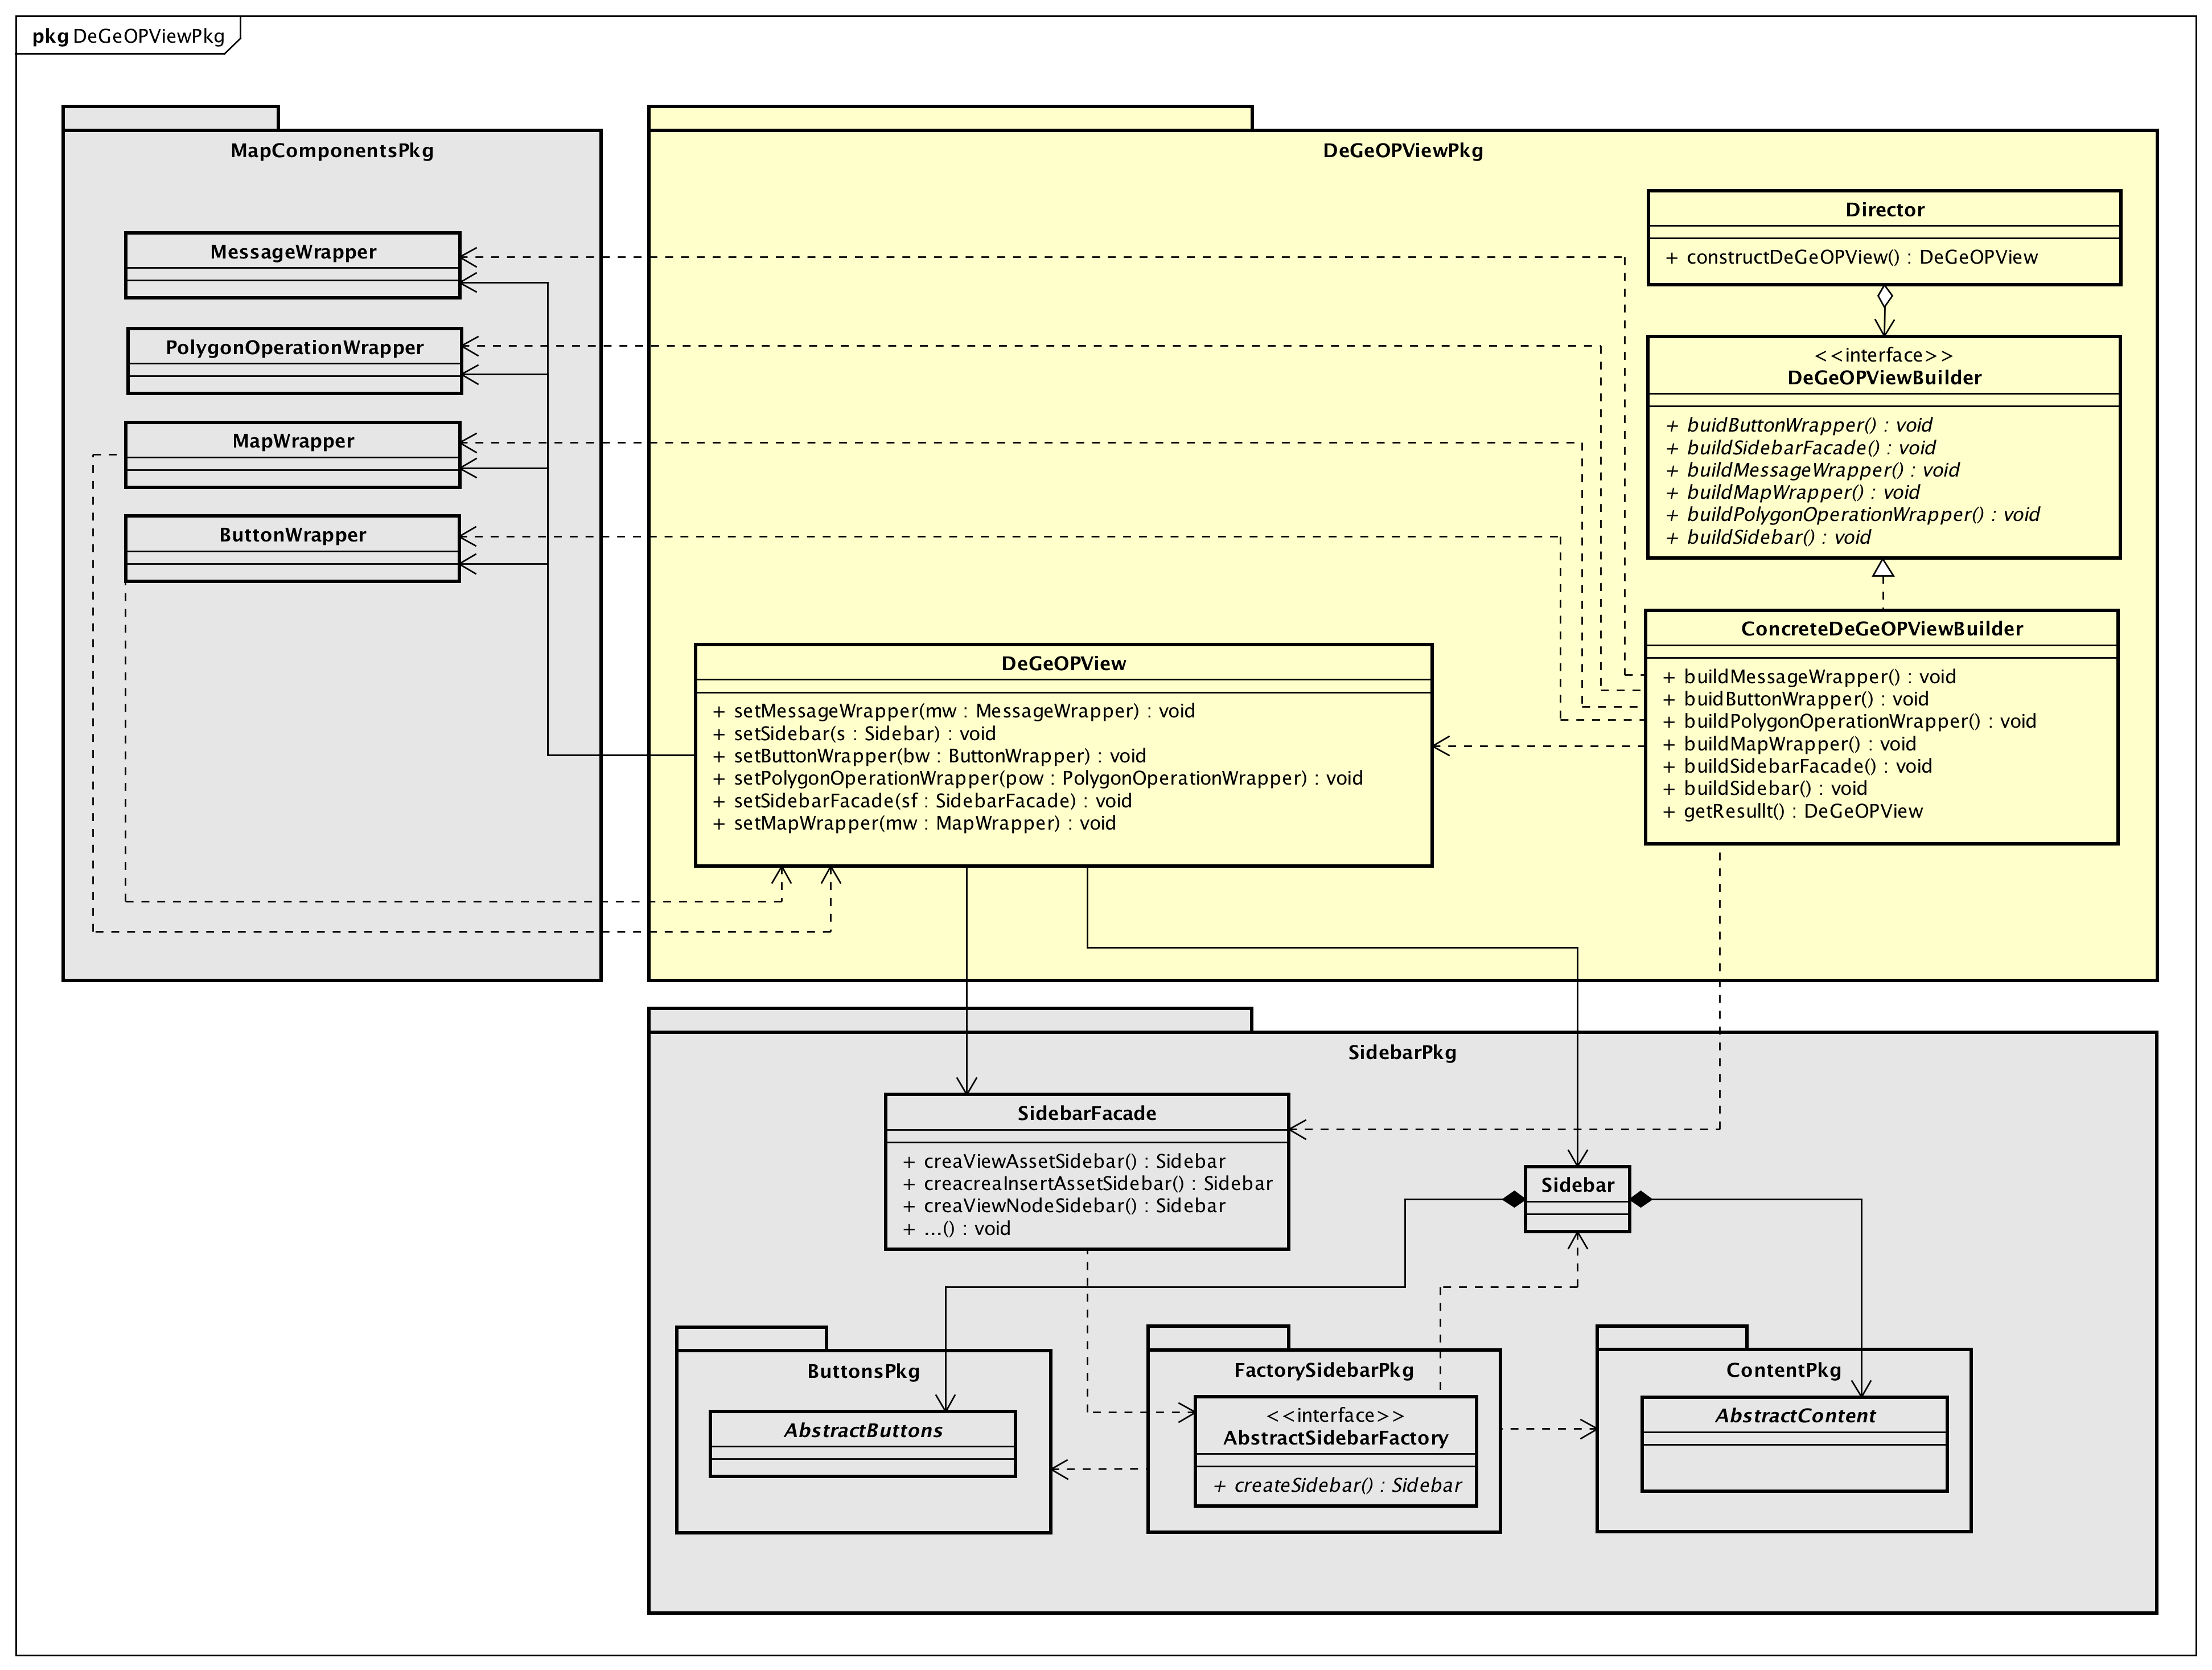
\includegraphics[width=\textwidth]{img/PkgDiagram/STDeGeOPViewPkg.png}
	\caption{Schema componente DeGeOP::ViewPkg::DeGeOPViewPkg}
\end{figure}
\subsubsection{Informazioni sul package}
\begin{itemize}
	\item \textbf{descrizione:} racchiude la componente principale della view;
	\item \textbf{padre:} \hyperref[pkg::ViewPkg]{ViewPkg};
	\item \textbf{interazioni con altri package:} 
	\begin{itemize}
		\item IN MapComponentsPkg: utilizzo di componenti grafiche;
		\item OUT MapComponentsPkg: utilizzo di componenti grafiche;
		\item OUT SidebarPkg: utilizzo della sidebar.
	\end{itemize}
	\item \textbf{classi contenute:}
	\begin{itemize}
		\item ConcreteDeGeOPViewBuilder;
		\item DeGeOPView;
		\item DeGeOPViewBuilder;
		\item Director.
	\end{itemize}
\end{itemize}
\subsubsection{Classi}
\paragraph{ConcreteDeGeOPViewBuilder}
\begin{itemize}
	\item \textbf{descrizione:} rappresenta un'implementazione di DeGeOPViewBuilder;
	\item \textbf{utilizzo:} i suoi metodi vengono invocati dal director per creare le varie componenti di DeGeOPView;
	\item \textbf{relazioni con altre classi:} 
	\begin{itemize}
		\item OUT MapWrapper.
	\end{itemize}
\end{itemize}
\paragraph{DeGeOPView}
\begin{itemize}
	\item \textbf{descrizione:} rappresenta l'oggetto grafico radice, che comprende l'intera View del prodotto;
	\item \textbf{utilizzo:} i suoi metodi setter sono richiamati da ConcreteDeGeOPViewBuilder per impostare i suoi campi dati. La classe effettua il subscribe sullo Store per ricevere gli aggiornamenti .
\end{itemize}
\paragraph{DeGeOPViewBuilder}
\begin{itemize}
	\item \textbf{descrizione:} interfaccia che rappresenta un builder per l'oggetto DeGeOPView;
	\item \textbf{utilizzo:} viene implementata per istanziare un builder concreto di DeGeOPView.
\end{itemize}
\paragraph{Director}
\begin{itemize}
	\item \textbf{descrizione:} rappresenta il director del design pattern builder usato per creare la View;
	\item \textbf{utilizzo:} è utilizzato per avviare la costruzione di DeGeOPView chiamando i metodi di un DeGeOPViewBuilder.
\end{itemize}
\newpage
\subsection{DeGeOP::ViewPkg::MapComponentsPkg}
\label{pkg::MapComponentsPkg}
\begin{figure}[H]
	\centering
	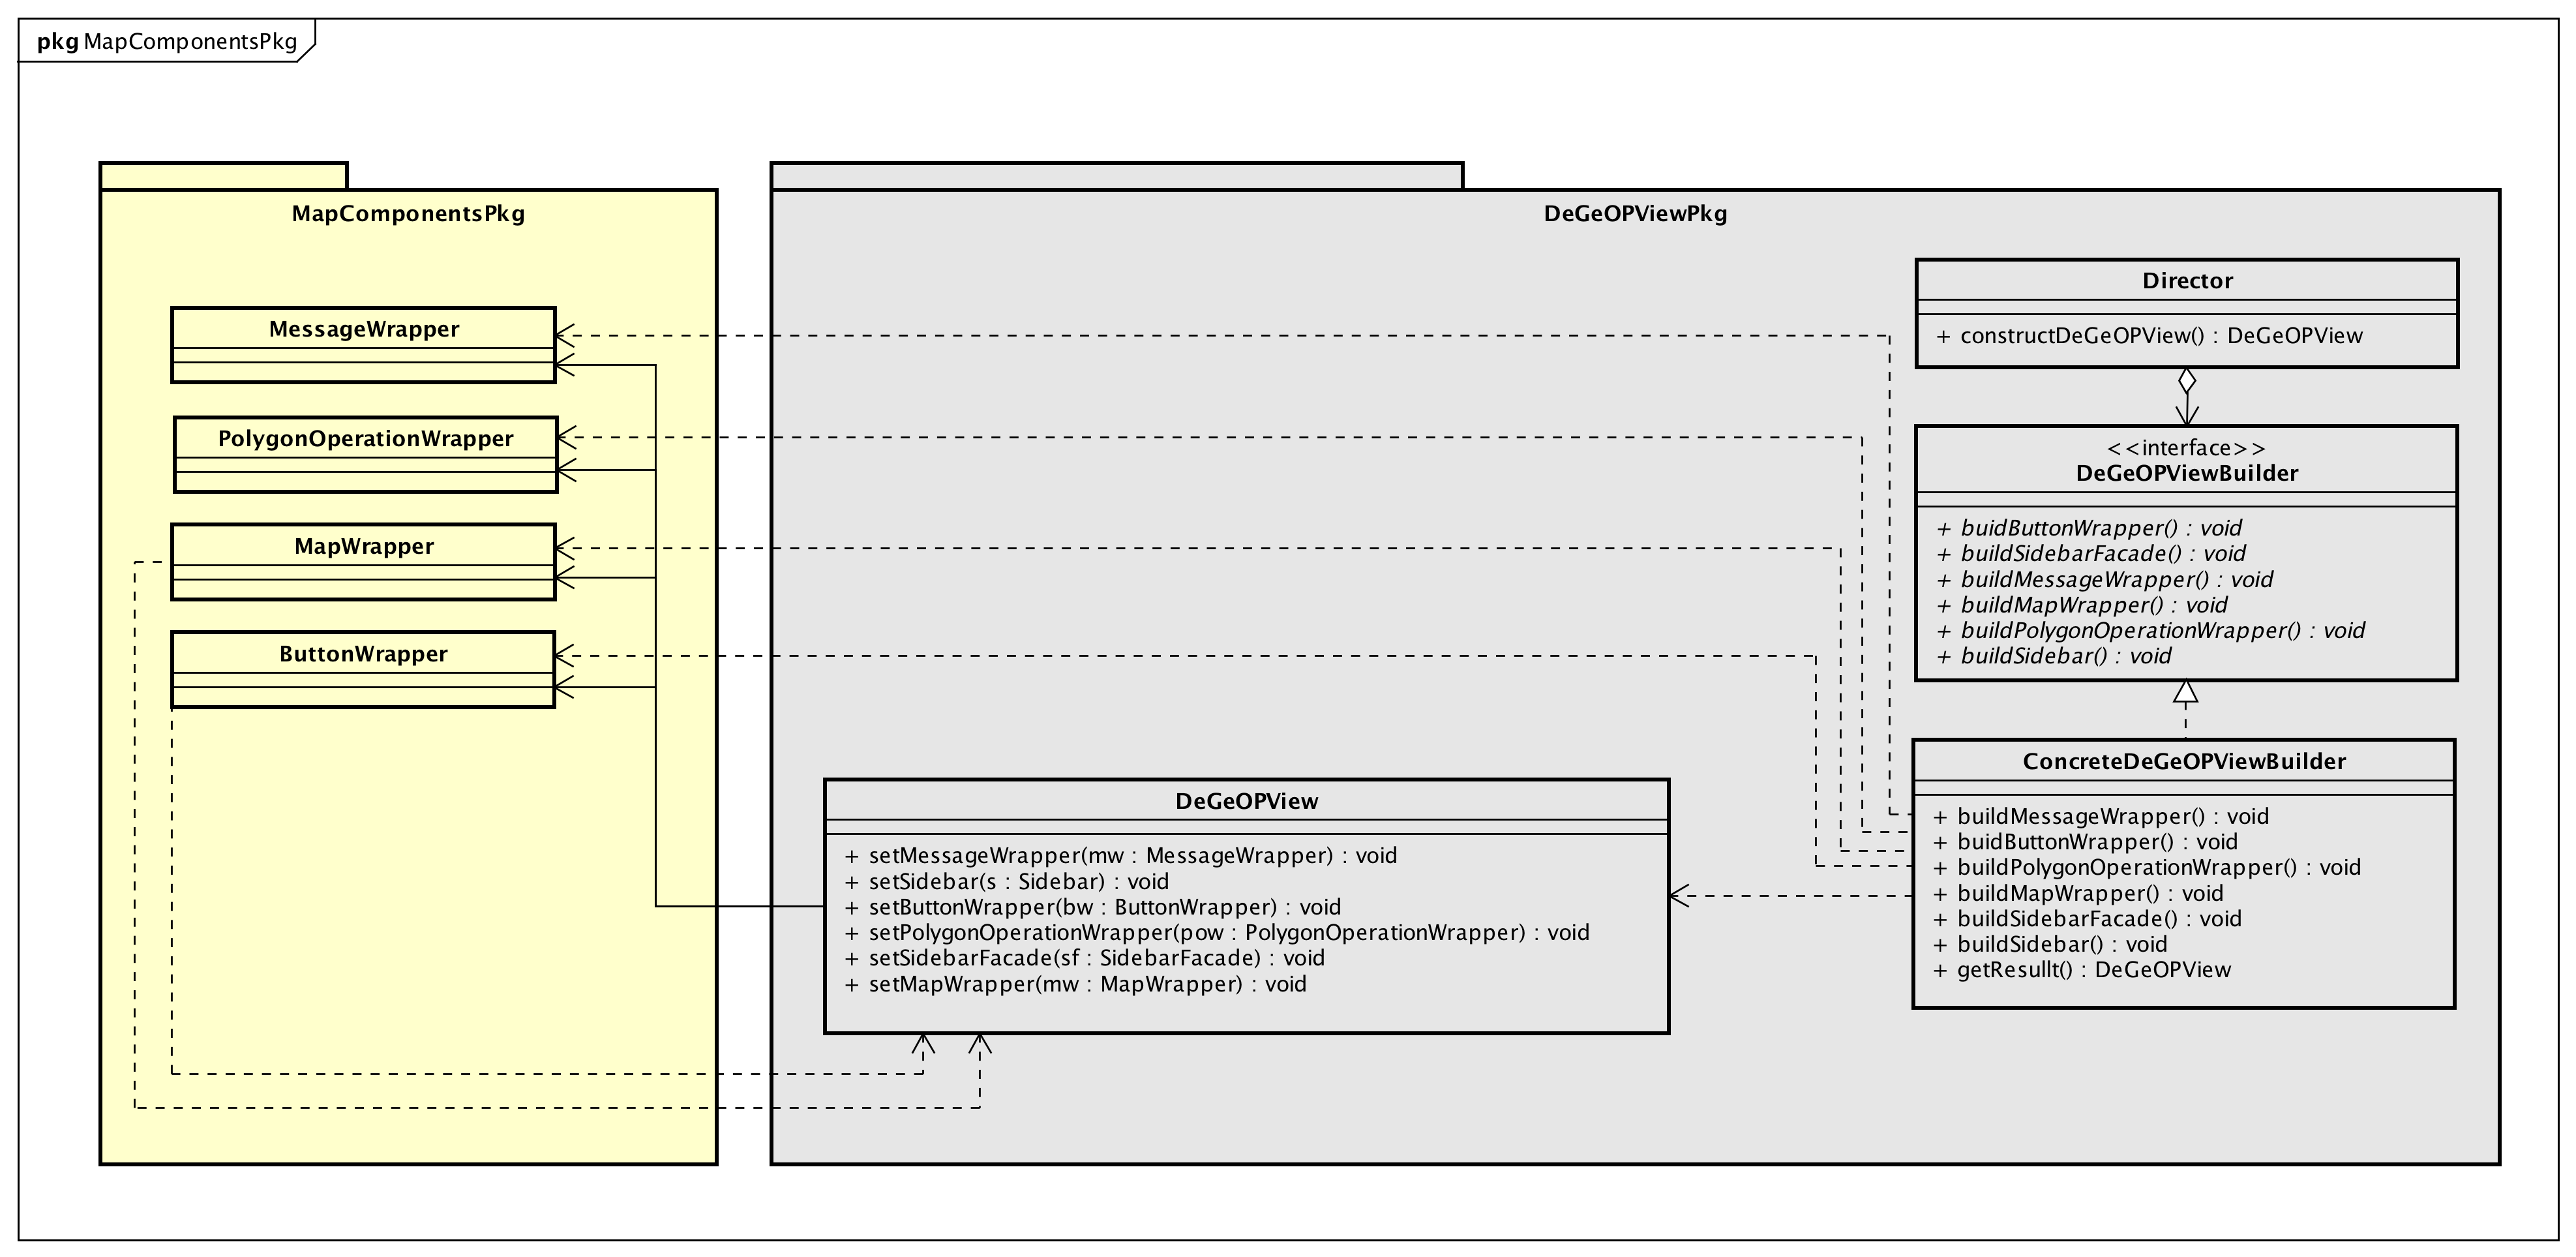
\includegraphics[width=\textwidth]{img/PkgDiagram/STMapComponentsPkg.png}
	\caption{Schema componente DeGeOP::ViewPkg::MapComponentsPkg}
\end{figure}
\subsubsection{Informazioni sul package}
\begin{itemize}
	\item \textbf{descrizione:} racchiude le componenti relative alla mappa e ai pulsanti sopra di essa;
	\item \textbf{padre:} \hyperref[pkg::ViewPkg]{ViewPkg};
	\item \textbf{interazioni con altri package:} 
	\begin{itemize}
		\item IN DeGeOPViewPkg: utilizzo di componenti grafiche;
		\item OUT DeGeOPViewPkg: utilizzo di componenti grafiche;
		\item OUT Openlayers: gestione mappa.
	\end{itemize}
	\item \textbf{classi contenute:}
	\begin{itemize}
		\item ButtonWrapper;
		\item MapWrapper;
		\item MessageWrapper;
		\item PolygonOperationWrapper.
	\end{itemize}
\end{itemize}
\subsubsection{Classi}
\paragraph{ButtonWrapper}
\begin{itemize}
	\item \textbf{descrizione:} rappresenta una classe wrapper per visualizzare una serie di bottoni con cui è possibile eseguire varie operazioni;
	\item \textbf{utilizzo:} viene utilizzato per mostrare sulla mappa una serie di bottoni.
\end{itemize}
\paragraph{MapWrapper}
\begin{itemize}
	\item \textbf{descrizione:} rappresenta una classe wrapper per visualizzare la mappa;
	\item \textbf{utilizzo:} viene utilizzata per visualizzare una mappa e permettere all'utente di interagire con essa;
	\item \textbf{relazioni con altre classi:} 
	\begin{itemize}
		\item IN ConcreteDeGeOPViewBuilder.
	\end{itemize}
\end{itemize}
\paragraph{MessageWrapper}
\begin{itemize}
	\item \textbf{descrizione:} rappresenta una classe wrapper per visualizzare un messaggio;
	\item \textbf{utilizzo:} viene utilizzato per mostrare messaggi di errore o di successo sulla mappa.
\end{itemize}
\paragraph{PolygonOperationWrapper}
\begin{itemize}
	\item \textbf{descrizione:} rappresenta una classe wrapper per visualizzare un bottone con cui è possibile effettuare operazioni sul perimetro di un poligono sulla mappa;
	\item \textbf{utilizzo:} invocando i suoi metodi è possibile iniziare a disegnare il poligono su mappa oppure cancellare l'ultimo segmento disegnato.
\end{itemize}
\newpage
\subsection{DeGeOP::ViewPkg::SidebarPkg}
\label{pkg::SidebarPkg}
\begin{figure}[H]
	\centering
	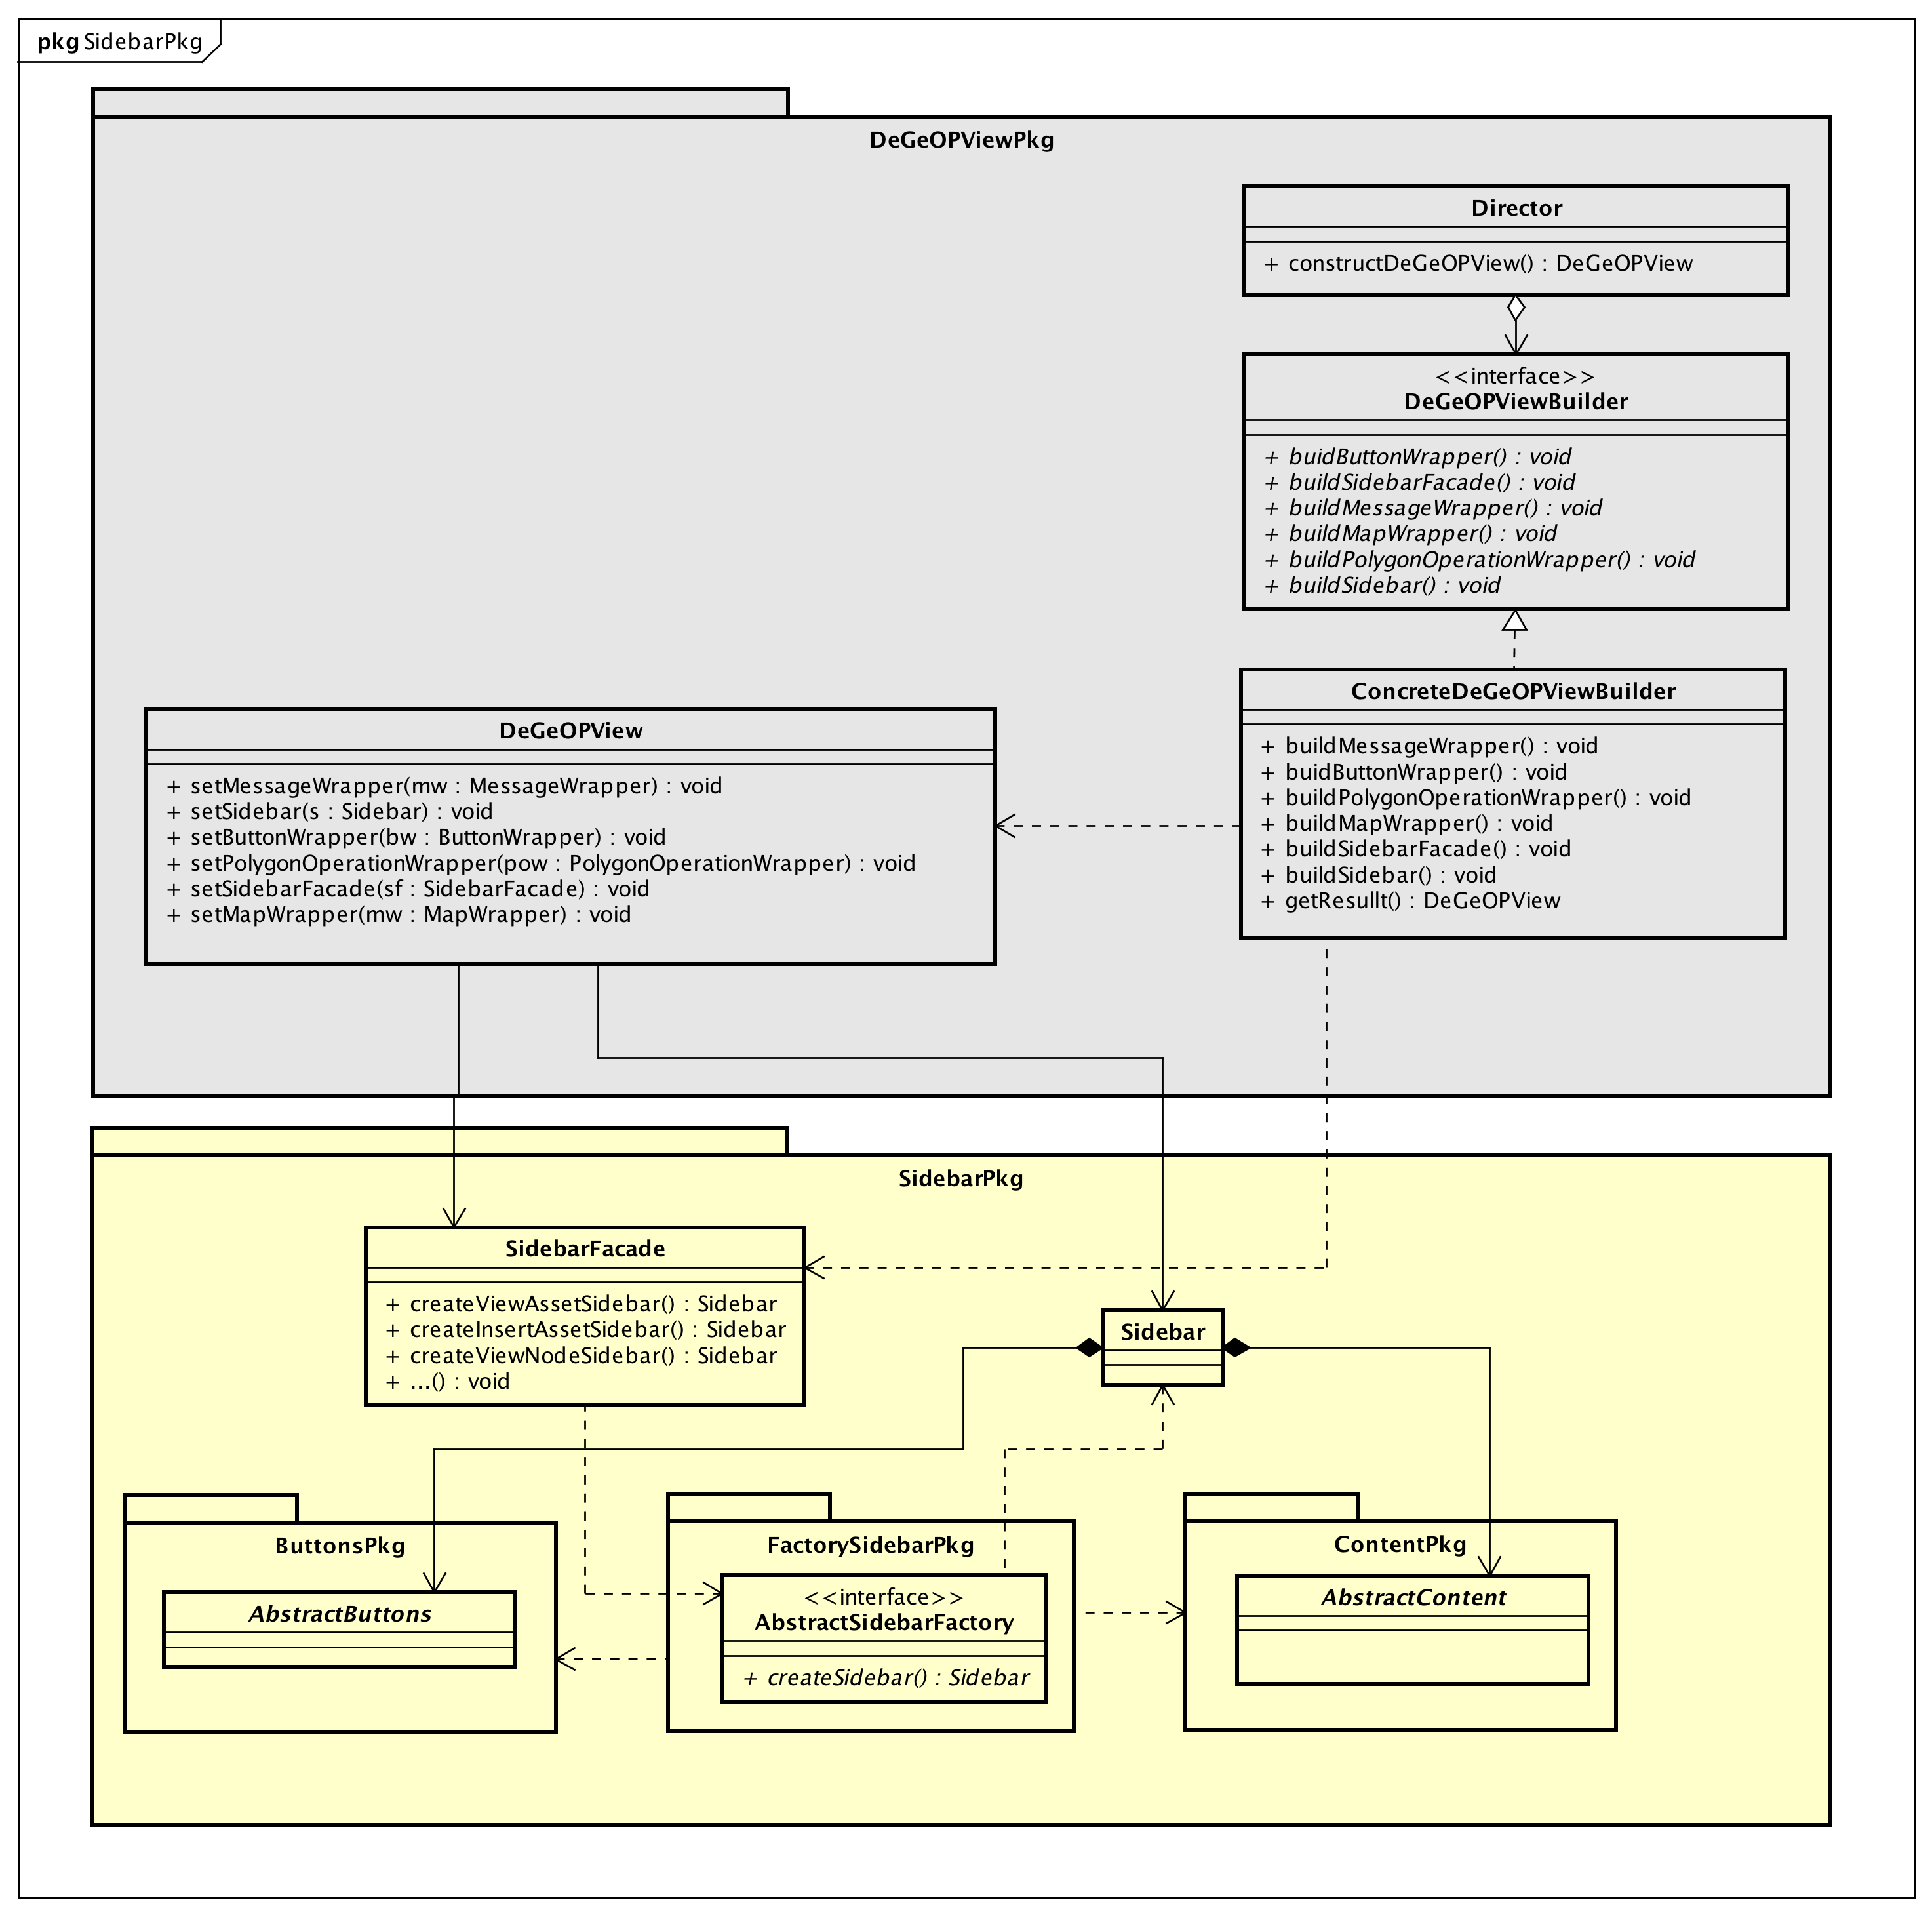
\includegraphics[width=\textwidth]{img/PkgDiagram/STSidebarPkg.png}
	\caption{Schema componente DeGeOP::ViewPkg::SidebarPkg}
\end{figure}
\subsubsection{Informazioni sul package}
\begin{itemize}
	\item \textbf{descrizione:} racchiude le componenti necessarie alla rappresentazione della sidebar;
	\item \textbf{padre:} \hyperref[pkg::ViewPkg]{ViewPkg};
	\item \textbf{package contenuti:}
	\begin{itemize}
		\item SidebarPkg::\hyperref[pkg::ButtonsPkg]{ButtonsPkg};
		\item SidebarPkg::\hyperref[pkg::ContentPkg]{ContentPkg};
		\item SidebarPkg::\hyperref[pkg::FactorySidebarPkg]{FactorySidebarPkg}.
	\end{itemize}
	\item \textbf{interazioni con altri package:} 
	\begin{itemize}
		\item IN DeGeOPViewPkg: utilizzo della sidebar.
	\end{itemize}
	\item \textbf{classi contenute:}
	\begin{itemize}
		\item Sidebar;
		\item SidebarFacade.
	\end{itemize}
\end{itemize}
\subsubsection{Classi}
\paragraph{Sidebar}
\begin{itemize}
	\item \textbf{descrizione:} rappresenta una sidebar contenente una serie di componenti grafiche;
	\item \textbf{utilizzo:} renderizza una sidebar composta da contenuto in cui l'utente può compilare i dati e da bottoni che permettono di eseguire varie operazioni, come ad esempio inserimenti e modifiche.
\end{itemize}
\paragraph{SidebarFacade}
\begin{itemize}
	\item \textbf{descrizione:} rappresenta un Facade tra DeGeOPView e Abstract;
	\item \textbf{utilizzo:} i suoi metodi vengono invocati per la creazione di Sidebar di vari tipologie senza che DeGeOPView necessiti di conoscere del tipo concreto delle Factory. Facade utilizza SidebarFactory concrete all'interno dei suoi metodi.
\end{itemize}
\newpage
\subsection{DeGeOP::ViewPkg::SidebarPkg::FactorySidebarPkg}
\label{pkg::FactorySidebarPkg}
\begin{figure}[H]
	\centering
	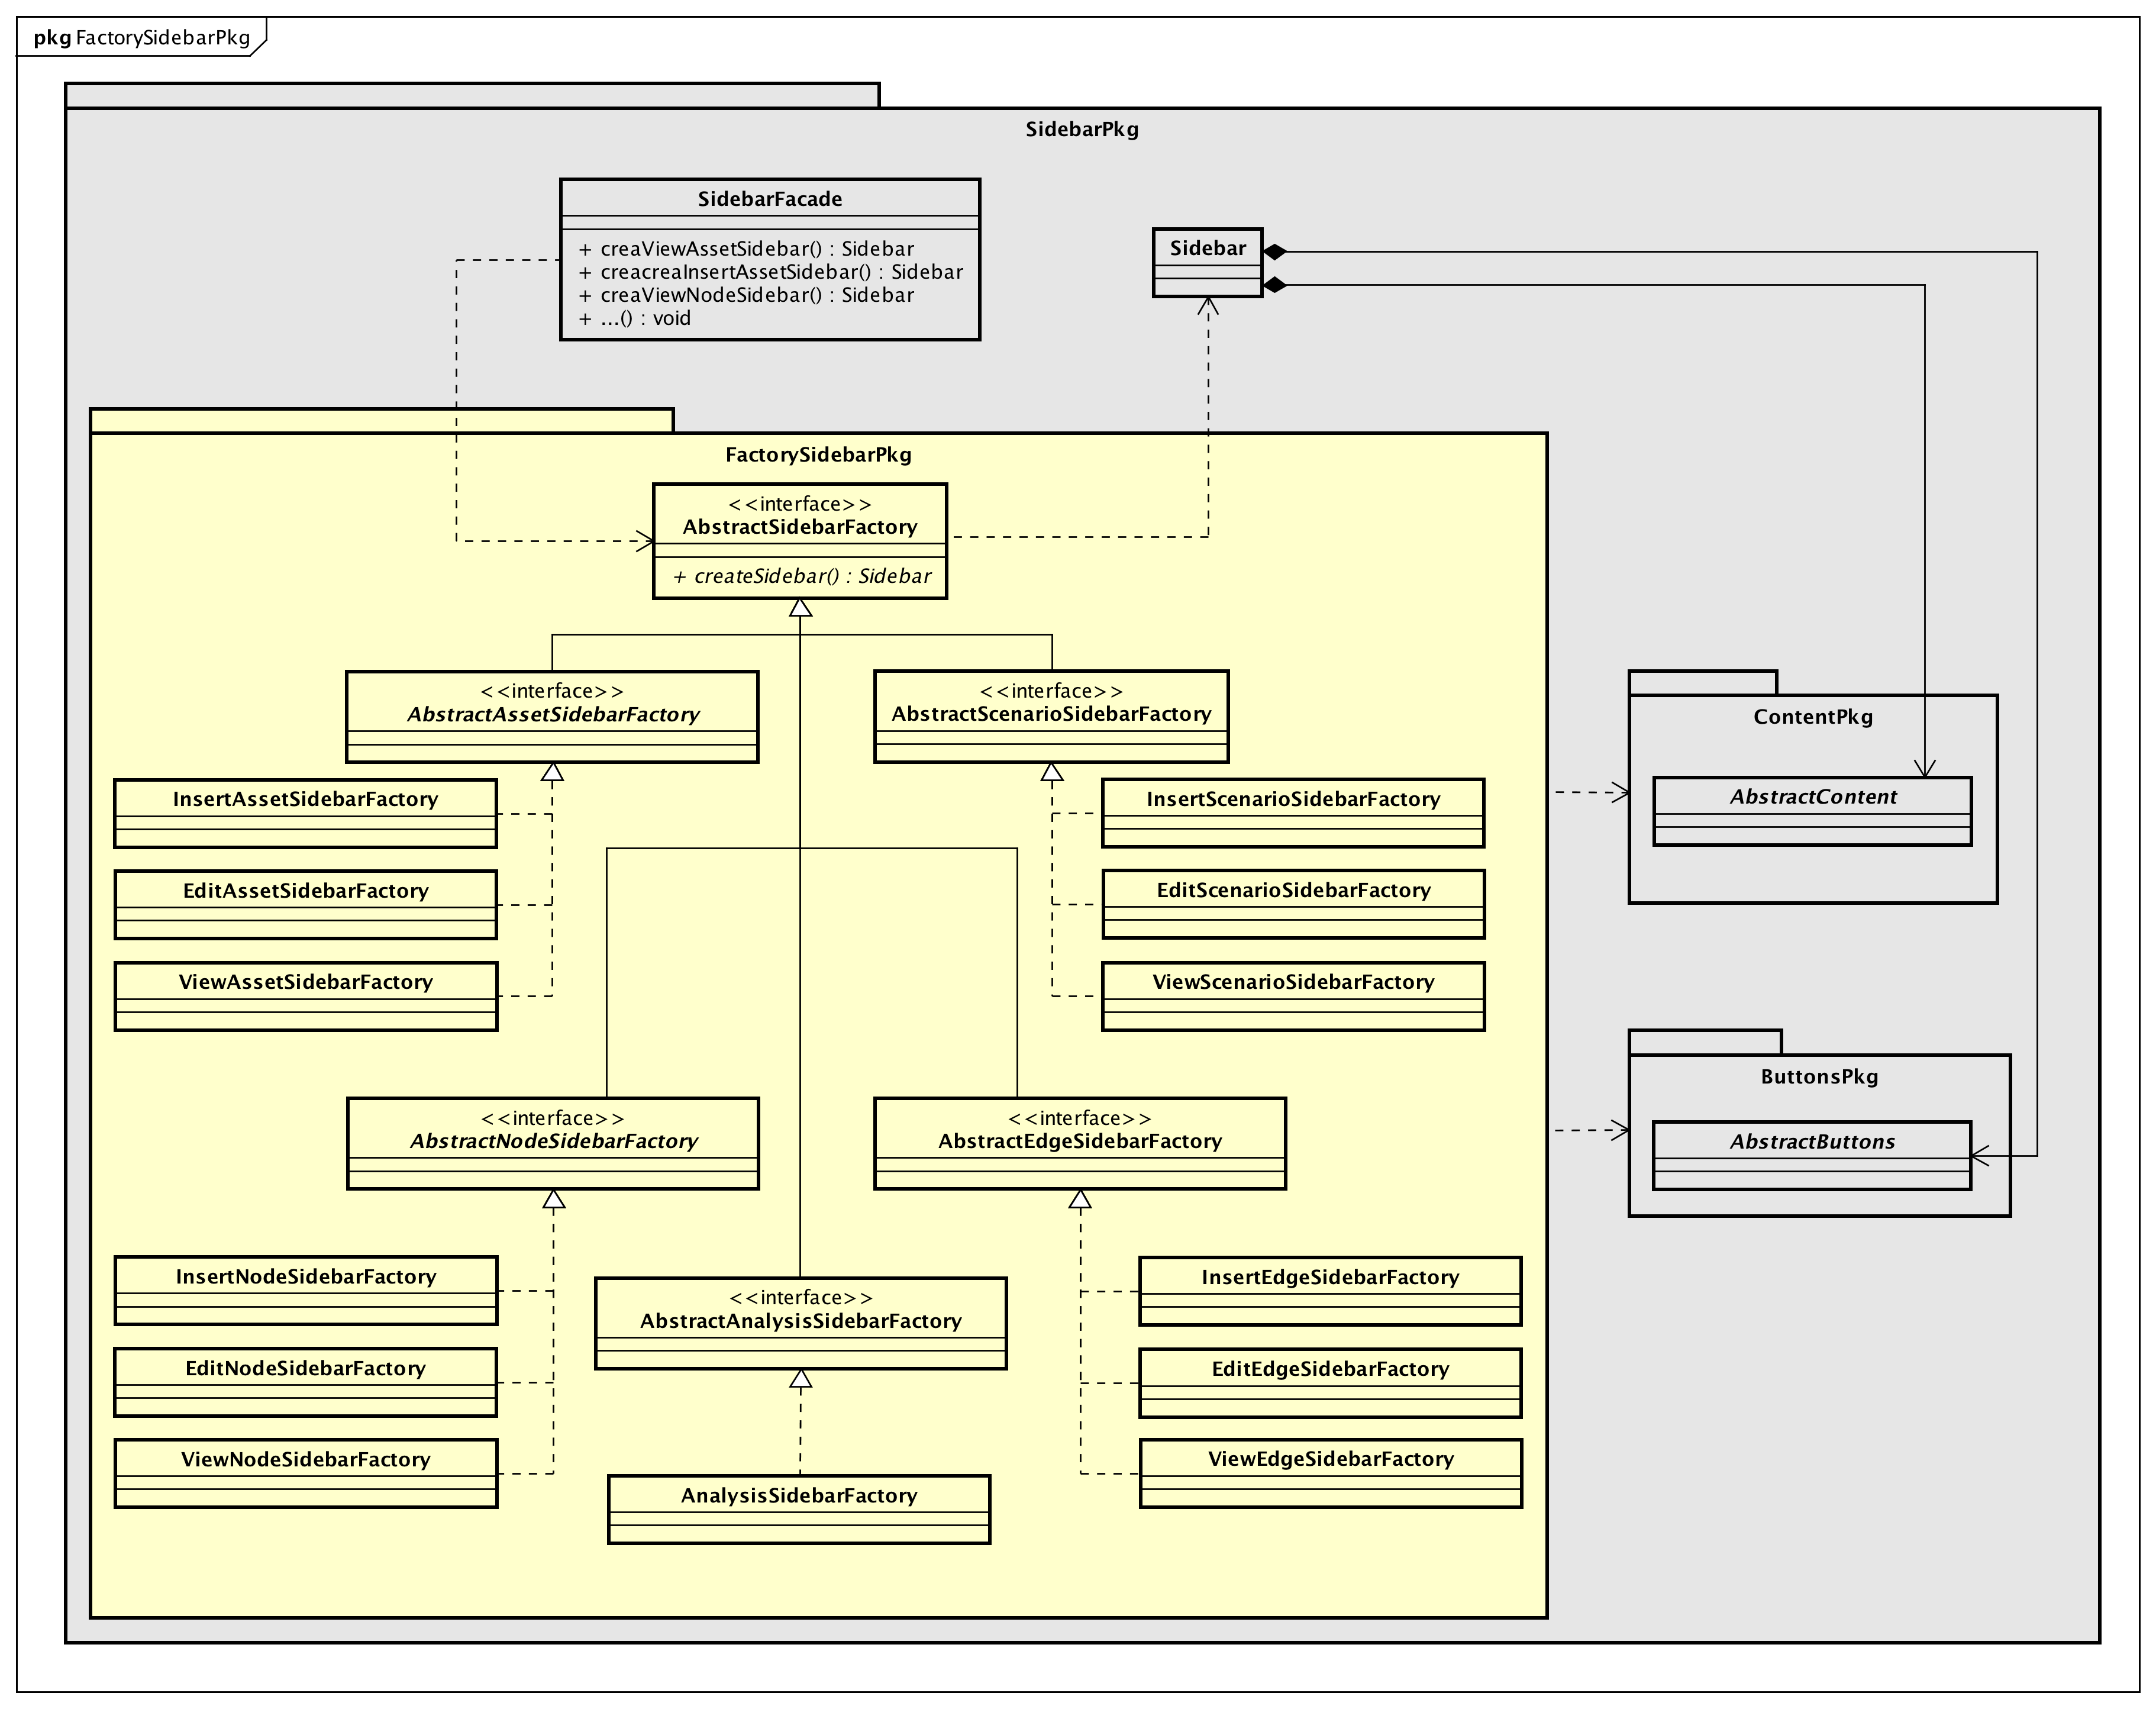
\includegraphics[width=\textwidth]{img/PkgDiagram/STFactorySidebarPkg.png}
	\caption{Schema componente DeGeOP::ViewPkg::SidebarPkg::FactorySidebarPkg}
\end{figure}
\subsubsection{Informazioni sul package}
\begin{itemize}
	\item \textbf{descrizione:} Racchiude le componenti Factory per la sidebar;
	\item \textbf{padre:} \hyperref[pkg::SidebarPkg]{SidebarPkg};
	\item \textbf{interazioni con altri package:} 
	\begin{itemize}
		\item OUT ContentPkg: creazione contenuto della sidebar.
	\end{itemize}
	\item \textbf{classi contenute:}
	\begin{itemize}
		\item AbstractAnalysisSidebarFactory;
		\item AbstractAssetSidebarFactory;
		\item AbstractEdgeSidebarFactory;
		\item AbstractNodeSidebarFactory;
		\item AbstractScenarioSidebarFactory;
		\item AbstractSidebarFactory;
		\item AnalysisSidebarFactory;
		\item EditAssetSidebarFactory;
		\item EditEdgeSidebarFactory;
		\item EditNodeSidebarFactory;
		\item EditScenarioSidebarFactory;
		\item InsertAssetSidebarFactory;
		\item InsertEdgeSidebarFactory;
		\item InsertNodeSidebarFactory;
		\item InsertScenarioSidebarFactory;
		\item ViewAssetSidebarFactory;
		\item ViewEdgeSidebarFactory;
		\item ViewNodeSidebarFactory;
		\item ViewScenarioSidebarFactory.
	\end{itemize}
\end{itemize}
\subsubsection{Classi}
\paragraph{AbstractAnalysisSidebarFactory}
\begin{itemize}
	\item \textbf{descrizione:} abstract factory relativa alla sidebar analisi di danno;
	\item \textbf{utilizzo:} viene usata come interfaccia di specializzazione fra abstractSidebar e le istanze di sidebar specifiche.
\end{itemize}
\paragraph{AbstractAssetSidebarFactory}
\begin{itemize}
	\item \textbf{descrizione:} abstract factory relativa alla sidebar asset;
	\item \textbf{utilizzo:}  viene usata come interfaccia di specializzazione fra abstractSidebar e le istanze di sidebar specifiche.
\end{itemize}
\paragraph{AbstractEdgeSidebarFactory}
\begin{itemize}
	\item \textbf{descrizione:} abstract factory relativa alla sidebar archi;
	\item \textbf{utilizzo:} viene usata come interfaccia di specializzazione fra abstractSidebar e le istanze di sidebar specifiche.
\end{itemize}
\paragraph{AbstractNodeSidebarFactory}
\begin{itemize}
	\item \textbf{descrizione:} abstract factory relativa alla sidebar nodi;
	\item \textbf{utilizzo:} viene usata come interfaccia di specializzazione fra abstractSidebar e le istanze di sidebar specifiche.
\end{itemize}
\paragraph{AbstractScenarioSidebarFactory}
\begin{itemize}
	\item \textbf{descrizione:} abstract factory relativa alla sidebar scenari;
	\item \textbf{utilizzo:} viene usata come interfaccia di specializzazione fra abstractSidebar e le istanze di sidebar specifiche.
\end{itemize}
\paragraph{AbstractSidebarFactory}
\begin{itemize}
	\item \textbf{descrizione:} una classe d'interfaccia rappresentante una sidebar con il relativo contenuto;
	\item \textbf{utilizzo:} è utilizzata da SidebarFacade per la creazione di Sidebar.
\end{itemize}
\paragraph{AnalysisSidebarFactory}
\begin{itemize}
	\item \textbf{descrizione:} rappresenta una factory concreta di una sidebar relativa alle analisi di danno;
	\item \textbf{utilizzo:} viene utilizzata da SidebarFacade per la creazione di Sidebar relativa alle analisi di danno.
\end{itemize}
\paragraph{EditAssetSidebarFactory}
\begin{itemize}
	\item \textbf{descrizione:} rappresenta una factory concreta di una sidebar relativa alla modifica di un asset;
	\item \textbf{utilizzo:} viene utilizzata da SidebarFacade per la creazione di Sidebar per la modifica di un asset.
\end{itemize}
\paragraph{EditEdgeSidebarFactory}
\begin{itemize}
	\item \textbf{descrizione:} rappresenta una factory concreta di una sidebar relativa alla modifica di un arco;
	\item \textbf{utilizzo:} viene utilizzata da SidebarFacade per la creazione di Sidebar per la modifica di un arco.
\end{itemize}
\paragraph{EditNodeSidebarFactory}
\begin{itemize}
	\item \textbf{descrizione:} rappresenta una factory concreta di una sidebar relativa all'inserimento di un nodo;
	\item \textbf{utilizzo:} viene utilizzata da SidebarFacade per la creazione di Sidebar per l'inserimento di un nodo.
\end{itemize}
\paragraph{EditScenarioSidebarFactory}
\begin{itemize}
	\item \textbf{descrizione:} rappresenta una factory concreta di una sidebar relativa all'inserimento di uno scenario di danno;
	\item \textbf{utilizzo:} viene utilizzata da SidebarFacade per la creazione di Sidebar per l'inserimento di uno scenario di danno.
\end{itemize}
\paragraph{InsertAssetSidebarFactory}
\begin{itemize}
	\item \textbf{descrizione:} rappresenta una factory concreta di una sidebar relativa all'inserimento di un asset;
	\item \textbf{utilizzo:} viene utilizzata da SidebarFacade per la creazione di Sidebar per l'inserimento di un asset.
\end{itemize}
\paragraph{InsertEdgeSidebarFactory}
\begin{itemize}
	\item \textbf{descrizione:} rappresenta una factory concreta di una sidebar relativa all'inserimento di un arco;
	\item \textbf{utilizzo:} viene utilizzata da SidebarFacade per la creazione di Sidebar per l'inserimento di un arco.
\end{itemize}
\paragraph{InsertNodeSidebarFactory}
\begin{itemize}
	\item \textbf{descrizione:} rappresenta una factory concreta di una sidebar relativa all'inserimento di un nodo;
	\item \textbf{utilizzo:} viene utilizzata da SidebarFacade per la creazione di Sidebar per l'inserimento di un nodo.
\end{itemize}
\paragraph{InsertScenarioSidebarFactory}
\begin{itemize}
	\item \textbf{descrizione:} rappresenta una factory concreta di una sidebar relativa all'inserimento di uno scenario di danno;
	\item \textbf{utilizzo:} viene utilizzata da SidebarFacade per la creazione di Sidebar per l'inserimento di uno scenario di danno.
\end{itemize}
\paragraph{ViewAssetSidebarFactory}
\begin{itemize}
	\item \textbf{descrizione:} rappresenta una factory concreta di una sidebar relativa alla visualizzazione di un asset;
	\item \textbf{utilizzo:} viene utilizzata da SidebarFacade per la creazione di Sidebar per la visualizzazione di un asset.
\end{itemize}
\paragraph{ViewEdgeSidebarFactory}
\begin{itemize}
	\item \textbf{descrizione:} rappresenta una factory concreta di una sidebar relativa alla visualizzazione di un arco;
	\item \textbf{utilizzo:} viene utilizzata da SidebarFacade per la creazione di Sidebar per la visualizzazione di un arco.
\end{itemize}
\paragraph{ViewNodeSidebarFactory}
\begin{itemize}
	\item \textbf{descrizione:} rappresenta una factory concreta di una sidebar relativa all'inserimento di un nodo;
	\item \textbf{utilizzo:} viene utilizzata da SidebarFacade per la creazione di Sidebar per l'inserimento di un nodo.
\end{itemize}
\paragraph{ViewScenarioSidebarFactory}
\begin{itemize}
	\item \textbf{descrizione:} rappresenta una factory concreta di una sidebar relativa all'inserimento di uno scenario di danno;
	\item \textbf{utilizzo:} viene utilizzata da SidebarFacade per la creazione di Sidebar per l'inserimento di uno scenario di danno.
\end{itemize}
\newpage
\subsection{DeGeOP::ViewPkg::SidebarPkg::ContentPkg}
\label{pkg::ContentPkg}
\begin{figure}[H]
	\centering
	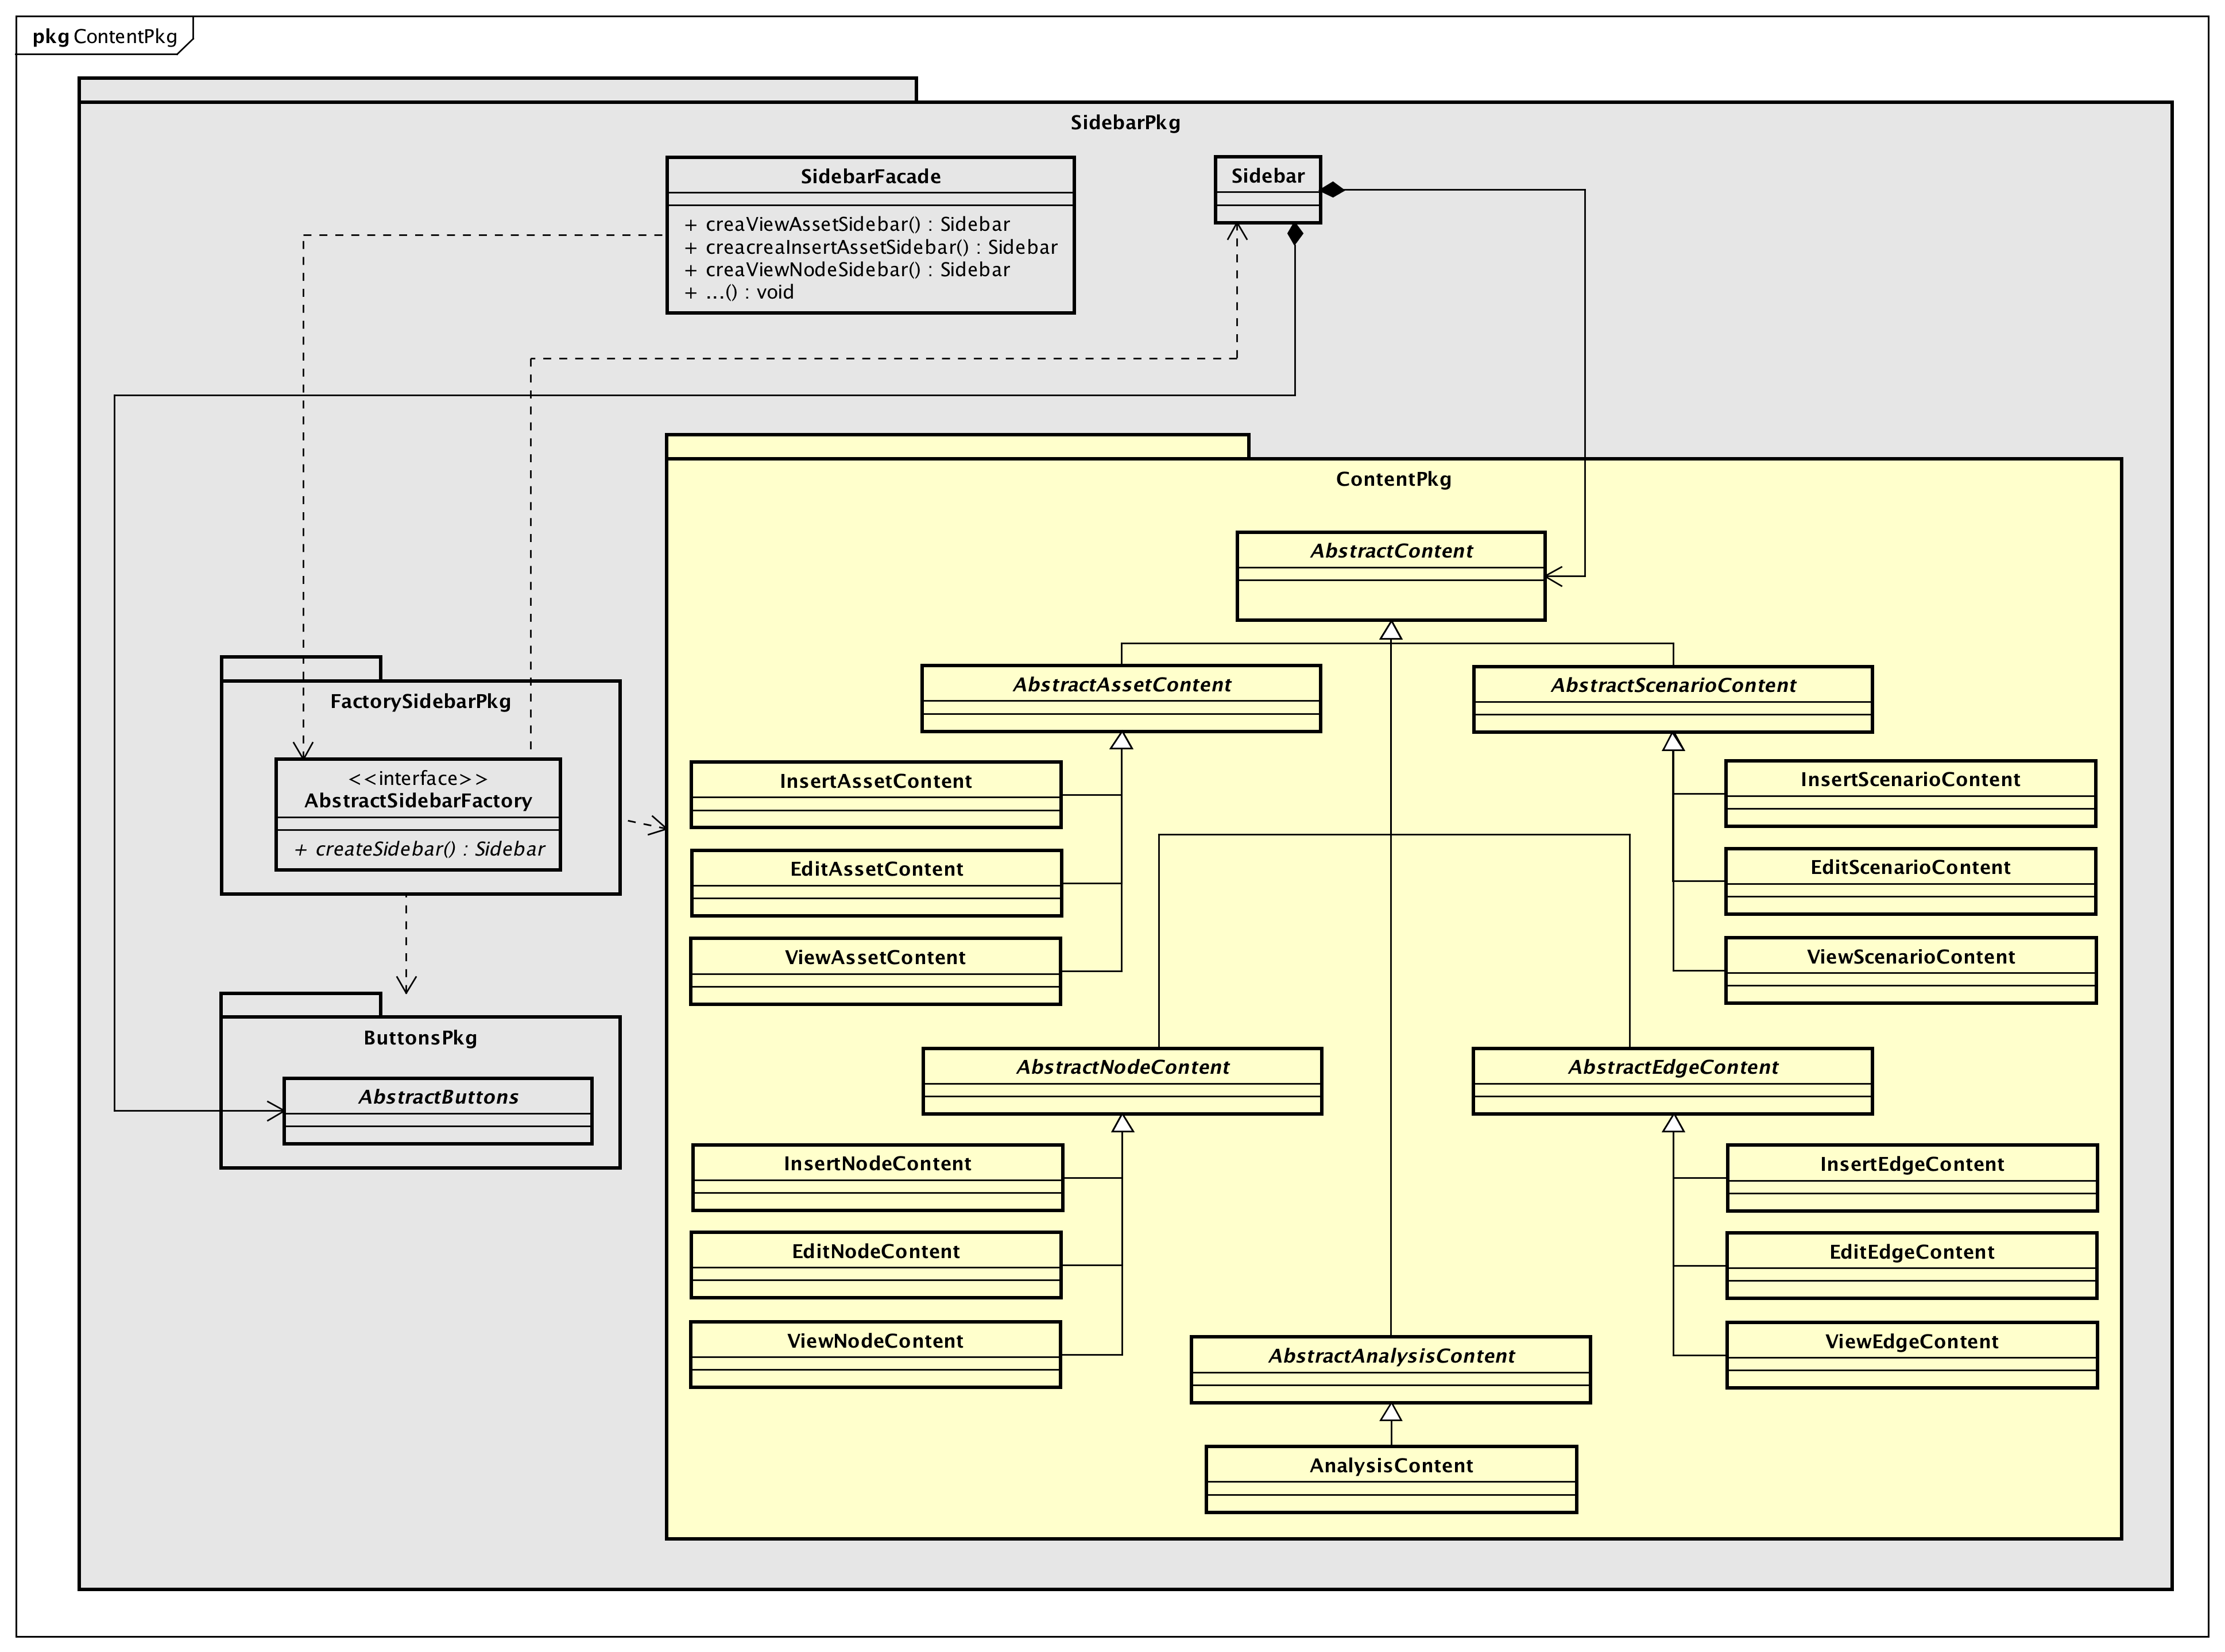
\includegraphics[width=\textwidth]{img/PkgDiagram/STContentPkg.png}
	\caption{Schema componente DeGeOP::ViewPkg::SidebarPkg::ContentPkg}
\end{figure}
\subsubsection{Informazioni sul package}
\begin{itemize}
	\item \textbf{descrizione:} racchiude le componenti che sono relative all'area informativa della Sidebar;
	\item \textbf{padre:} \hyperref[pkg::SidebarPkg]{SidebarPkg};
	\item \textbf{interazioni con altri package:} 
	\begin{itemize}
		\item IN FactorySidebarPkg: creazione contenuto della sidebar;
		\item OUT React-color: visualizzazione palette colori.
	\end{itemize}
	\item \textbf{classi contenute:}
	\begin{itemize}
		\item AbstractAnalysisContent;
		\item AbstractAssetContent;
		\item AbstractContent;
		\item AbstractEdgeContent;
		\item AbstractNodeContent;
		\item AbstractScenarioContent;
		\item AnalysisContent;
		\item EditAssetContent;
		\item EditEdgeContent;
		\item EditNodeContent;
		\item EditScenarioContent;
		\item InsertAssetContent;
		\item InsertEdgeContent;
		\item InsertNodeContent;
		\item InsertScenarioContent;
		\item ViewAssetContent;
		\item ViewEdgeContent;
		\item ViewNodeContent;
		\item ViewScenarioContent.
	\end{itemize}
\end{itemize}
\subsubsection{Classi}
\paragraph{AbstractAnalysisContent}
\begin{itemize}
	\item \textbf{descrizione:} una classe astratta rappresentante il contenuto della sidebar durante le operazioni sulle analisi;
	\item \textbf{utilizzo:} viene usata come interfaccia di specializzazione fra abstractContent e le istanze di contenuti specifiche.
\end{itemize}
\paragraph{AbstractAssetContent}
\begin{itemize}
	\item \textbf{descrizione:} una classe astratta rappresentante il contenuto della sidebar durante le operazioni sugli asset;
	\item \textbf{utilizzo:} viene usata come interfaccia di specializzazione fra abstractContent e le istanze di contenuti specifiche.
\end{itemize}
\paragraph{AbstractContent}
\begin{itemize}
	\item \textbf{descrizione:} una classe d'interfaccia rappresentante il contenuto dell'area informativa nella sidebar;
	\item \textbf{utilizzo:} viene riferita da sidebar in quanto è una delle sue componenti.
\end{itemize}
\paragraph{AbstractEdgeContent}
\begin{itemize}
	\item \textbf{descrizione:} una classe astratta rappresentante il contenuto della sidebar durante le operazioni sugli archi;
	\item \textbf{utilizzo:} viene usata come interfaccia di specializzazione fra abstractContent e le istanze di contenuti specifiche.
\end{itemize}
\paragraph{AbstractNodeContent}
\begin{itemize}
	\item \textbf{descrizione:} una classe astratta rappresentante il contenuto della sidebar durante le operazioni sui nodi;
	\item \textbf{utilizzo:} viene usata come interfaccia di specializzazione fra abstractContent e le istanze di contenuti specifiche.
\end{itemize}
\paragraph{AbstractScenarioContent}
\begin{itemize}
	\item \textbf{descrizione:} una classe astratta rappresentante il contenuto della sidebar durante le operazioni sugli scenari;
	\item \textbf{utilizzo:} viene usata come interfaccia di specializzazione fra abstractContent e le istanze di contenuti specifiche.
\end{itemize}
\paragraph{AnalysisContent}
\begin{itemize}
	\item \textbf{descrizione:} rappresenta il contenuto della sidebar relativa all'analisi di danno;
	\item \textbf{utilizzo:} viene creata da AnalysisSidebarFactory .
\end{itemize}
\paragraph{EditAssetContent}
\begin{itemize}
	\item \textbf{descrizione:} rappresenta il contenuto della sidebar relativa alla modifica di un asset;
	\item \textbf{utilizzo:} viene creata da EditAssetSidebarFactory .
\end{itemize}
\paragraph{EditEdgeContent}
\begin{itemize}
	\item \textbf{descrizione:} rappresenta il contenuto della sidebar relativa alla modifica di un arco;
	\item \textbf{utilizzo:} viene creata da EditEdgeSidebarFactory .
\end{itemize}
\paragraph{EditNodeContent}
\begin{itemize}
	\item \textbf{descrizione:} rappresenta il contenuto della sidebar relativa alla modifica di un nodo;
	\item \textbf{utilizzo:} viene creata da EditNodeSidebarFactory .
\end{itemize}
\paragraph{EditScenarioContent}
\begin{itemize}
	\item \textbf{descrizione:} rappresenta il contenuto della Sidebar relativa alla modifica di uno scenario di danno;
	\item \textbf{utilizzo:} viene creata da EditScenarioSidebarFactory .
\end{itemize}
\paragraph{InsertAssetContent}
\begin{itemize}
	\item \textbf{descrizione:} rappresenta il contenuto della sidebar relativa all'inserimento di un asset;
	\item \textbf{utilizzo:} viene creata da InsertAssetSidebarFactory .
\end{itemize}
\paragraph{InsertEdgeContent}
\begin{itemize}
	\item \textbf{descrizione:} rappresenta il contenuto della sidebar relativa all'inserimento di un arco;
	\item \textbf{utilizzo:} viene creata da InsertEdgeSidebarFactory .
\end{itemize}
\paragraph{InsertNodeContent}
\begin{itemize}
	\item \textbf{descrizione:} rappresenta il contenuto della sidebar relativa all'inserimento di un nodo;
	\item \textbf{utilizzo:} viene creata da InsertNodeSidebarFactory .
\end{itemize}
\paragraph{InsertScenarioContent}
\begin{itemize}
	\item \textbf{descrizione:} rappresenta il contenuto della Sidebar relativa all'inserimento di uno scenario di danno;
	\item \textbf{utilizzo:} viene creata da InsertScenarioSidebarFactory .
\end{itemize}
\paragraph{ViewAssetContent}
\begin{itemize}
	\item \textbf{descrizione:} rappresenta il contenuto della sidebar relativa alla visualizzazione di un asset;
	\item \textbf{utilizzo:} viene creata da ViewAssetSidebarFactory .
\end{itemize}
\paragraph{ViewEdgeContent}
\begin{itemize}
	\item \textbf{descrizione:} rappresenta il contenuto della sidebar relativa alla visualizzazione di un arco;
	\item \textbf{utilizzo:} viene creata da ViewEdgeSidebarFactory .
\end{itemize}
\paragraph{ViewNodeContent}
\begin{itemize}
	\item \textbf{descrizione:} rappresenta il contenuto della sidebar relativa alla visualizzazione di un ndo;
	\item \textbf{utilizzo:} viene creata da ViewNodeSidebarFactory .
\end{itemize}
\paragraph{ViewScenarioContent}
\begin{itemize}
	\item \textbf{descrizione:} rappresenta il contenuto della Sidebar relativa alla visualizzazione di uno scenario di danno;
	\item \textbf{utilizzo:} viene creata da ViewScenarioSidebarFactory .
\end{itemize}
\newpage
\subsection{DeGeOP::ViewPkg::SidebarPkg::ButtonsPkg}
\label{pkg::ButtonsPkg}
\begin{figure}[H]
	\centering
	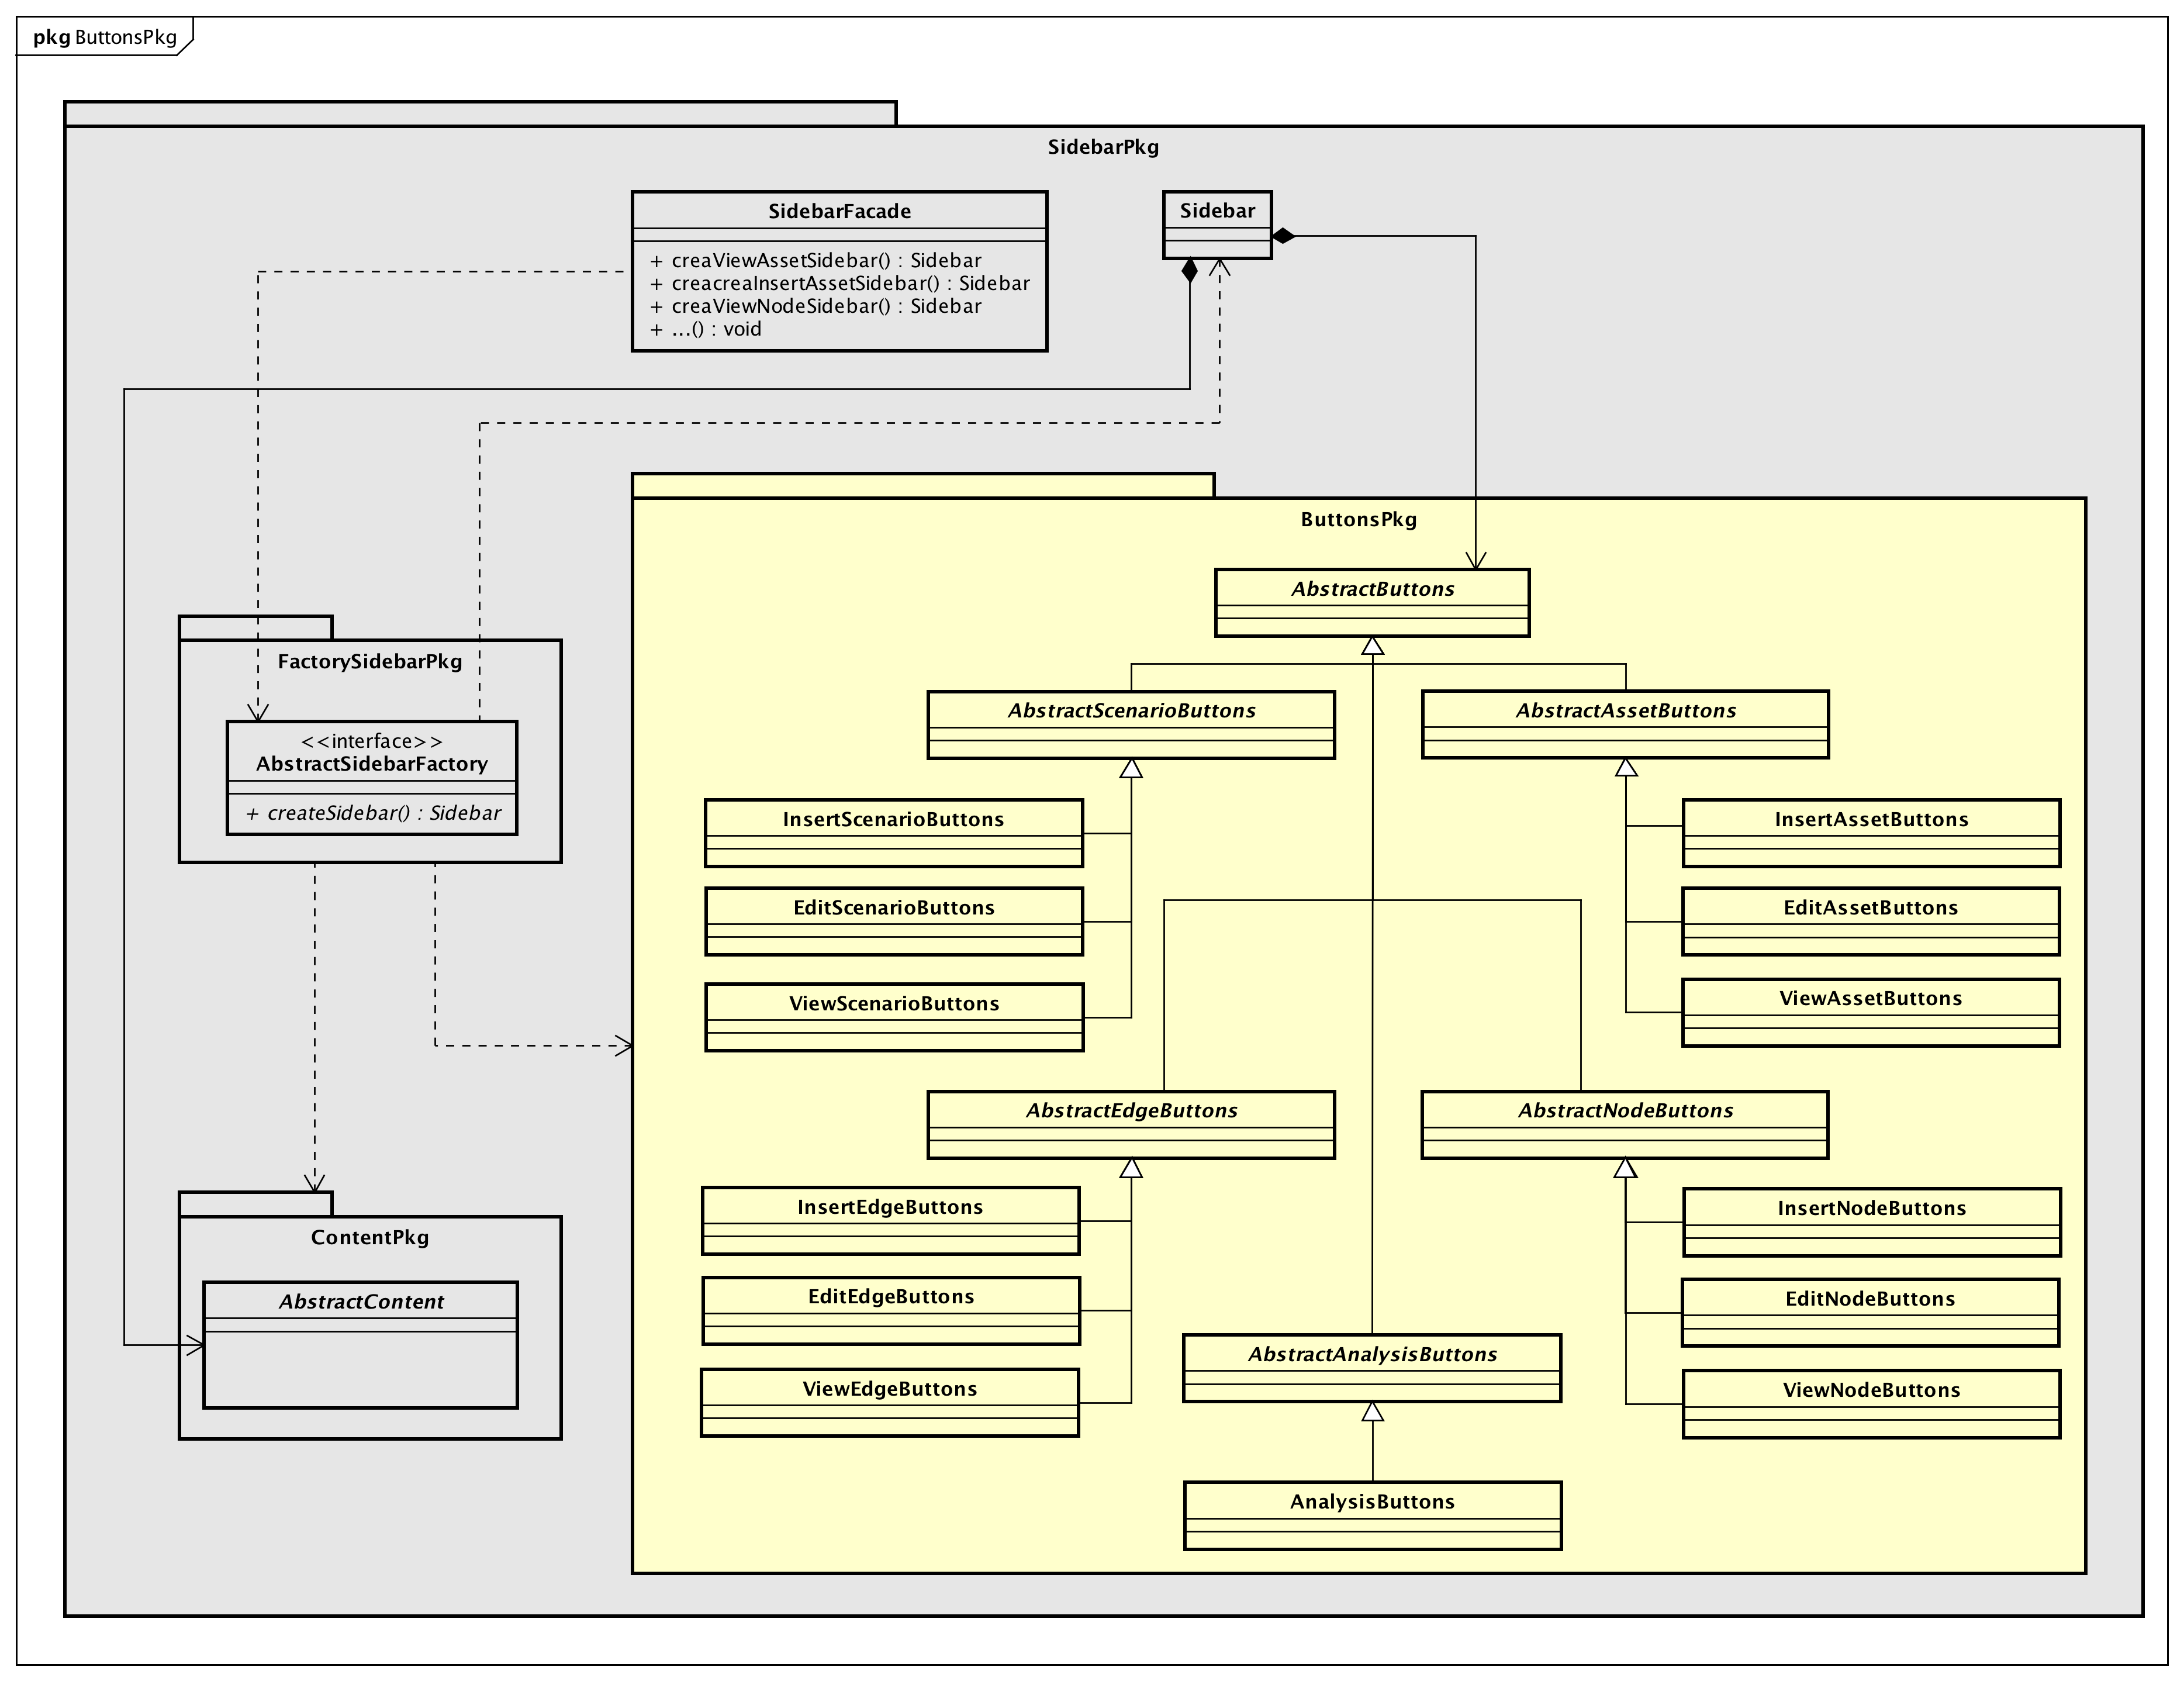
\includegraphics[width=\textwidth]{img/PkgDiagram/STButtonsPkg.png}
	\caption{Schema componente DeGeOP::ViewPkg::SidebarPkg::ButtonsPkg}
\end{figure}
\subsubsection{Informazioni sul package}
\begin{itemize}
	\item \textbf{descrizione:} racchiude le componenti che sono relative all'area con i bottoni della Sidebar;
	\item \textbf{padre:} \hyperref[pkg::SidebarPkg]{SidebarPkg};
	\item \textbf{classi contenute:}
	\begin{itemize}
		\item AbstractAnalysisButtons;
		\item AbstractAssetButtons;
		\item AbstractButtons;
		\item AbstractEdgeButtons;
		\item AbstractNodeButtons;
		\item AbstractScenarioButtons;
		\item AnalysisButtons;
		\item EditAssetButtons;
		\item EditEdgeButtons;
		\item EditNodeButtons;
		\item EditScenarioButtons;
		\item InsertAssetButtons;
		\item InsertEdgeButtons;
		\item InsertNodeButtons;
		\item InsertScenarioButtons;
		\item ViewAssetButtons;
		\item ViewEdgeButtons;
		\item ViewNodeButtons;
		\item ViewScenarioButtons.
	\end{itemize}
\end{itemize}
\subsubsection{Classi}
\paragraph{AbstractAnalysisButtons}
\begin{itemize}
	\item \textbf{descrizione:} una classe astratta rappresentante i bottoni della sidebar durante le operazioni sulle analisi;
	\item \textbf{utilizzo:} viene usata come interfaccia di specializzazione fra abstractButtons e le istanze di bottoni specifiche.
\end{itemize}
\paragraph{AbstractAssetButtons}
\begin{itemize}
	\item \textbf{descrizione:} una classe astratta rappresentante i bottoni della sidebar durante le operazioni sugli asset;
	\item \textbf{utilizzo:} viene usata come interfaccia di specializzazione fra abstractButtons e le istanze di bottoni specifiche.
\end{itemize}
\paragraph{AbstractButtons}
\begin{itemize}
	\item \textbf{descrizione:} una classe d'interfaccia rappresentante i bottoni inseriti nella sidebar;
	\item \textbf{utilizzo:} viene riferita da sidebar in quanto è una delle sue componenti.
\end{itemize}
\paragraph{AbstractEdgeButtons}
\begin{itemize}
	\item \textbf{descrizione:} una classe astratta rappresentante i bottoni della sidebar durante le operazioni sugli archi
	;
	\item \textbf{utilizzo:} viene usata come interfaccia di specializzazione fra abstractButtons e le istanze di bottoni specifiche.
\end{itemize}
\paragraph{AbstractNodeButtons}
\begin{itemize}
	\item \textbf{descrizione:} una classe astratta rappresentante i bottoni della sidebar durante le operazioni sui nodi
	;
	\item \textbf{utilizzo:} viene usata come interfaccia di specializzazione fra abstractButtons e le istanze di bottoni specifiche.
\end{itemize}
\paragraph{AbstractScenarioButtons}
\begin{itemize}
	\item \textbf{descrizione:} una classe astratta rappresentante i bottoni della sidebar durante le operazioni sugli scenari;
	\item \textbf{utilizzo:} viene usata come interfaccia di specializzazione fra abstractButtons e le istanze di bottoni specifiche.
\end{itemize}
\paragraph{AnalysisButtons}
\begin{itemize}
	\item \textbf{descrizione:} rappresenta i bottoni della sidebar relativi all'analisi di danno;
	\item \textbf{utilizzo:} viene creata da AnalysisFactory.
\end{itemize}
\paragraph{EditAssetButtons}
\begin{itemize}
	\item \textbf{descrizione:} rappresenta i bottoni della sidebar relativi alla modifica di un asset;
	\item \textbf{utilizzo:} viene creata da EditAssetFactory.
\end{itemize}
\paragraph{EditEdgeButtons}
\begin{itemize}
	\item \textbf{descrizione:} rappresenta i bottoni della sidebar relativi alla modifica di un arco;
	\item \textbf{utilizzo:} viene creata da EditEdgeFactory.
\end{itemize}
\paragraph{EditNodeButtons}
\begin{itemize}
	\item \textbf{descrizione:} rappresenta i bottoni della sidebar relativi alla modifica di un nodo;
	\item \textbf{utilizzo:} viene creata da EditNodeFactory.
\end{itemize}
\paragraph{EditScenarioButtons}
\begin{itemize}
	\item \textbf{descrizione:} rappresenta i bottoni della sidebar relativi alla modifica di uno scenario di danno;
	\item \textbf{utilizzo:} viene creata da EditScenarioFactory.
\end{itemize}
\paragraph{InsertAssetButtons}
\begin{itemize}
	\item \textbf{descrizione:} rappresenta i bottoni della sidebar relativi all'inserimento di un asset;
	\item \textbf{utilizzo:} viene creata da InsertAssetFactory.
\end{itemize}
\paragraph{InsertEdgeButtons}
\begin{itemize}
	\item \textbf{descrizione:} rappresenta i bottoni della sidebar relativi all'inserimento di un arco;
	\item \textbf{utilizzo:} viene creata da InsertEdgeFactory.
\end{itemize}
\paragraph{InsertNodeButtons}
\begin{itemize}
	\item \textbf{descrizione:} rappresenta i bottoni della sidebar relativi all'inserimento di un nodo;
	\item \textbf{utilizzo:} viene creata da InsertNodeFactory.
\end{itemize}
\paragraph{InsertScenarioButtons}
\begin{itemize}
	\item \textbf{descrizione:} rappresenta i bottoni della sidebar relativa all'inserimento di uno scenario di danno;
	\item \textbf{utilizzo:} viene creata da InsertScenarioFactory.
\end{itemize}
\paragraph{ViewAssetButtons}
\begin{itemize}
	\item \textbf{descrizione:} rappresenta i bottoni della sidebar relativi alla visualizzazione di un asset;
	\item \textbf{utilizzo:} viene creata da ViewAssetFactory.
\end{itemize}
\paragraph{ViewEdgeButtons}
\begin{itemize}
	\item \textbf{descrizione:} rappresenta i bottoni della sidebar relativi alla visualizzazione di un arco;
	\item \textbf{utilizzo:} viene creata da ViewEdgeFactory.
\end{itemize}
\paragraph{ViewNodeButtons}
\begin{itemize}
	\item \textbf{descrizione:} rappresenta i bottoni della sidebar relativi alla visualizzazione di un nodo;
	\item \textbf{utilizzo:} viene creata da ViewNodeFactory.
\end{itemize}
\paragraph{ViewScenarioButtons}
\begin{itemize}
	\item \textbf{descrizione:} rappresenta i bottoni della sidebar relativi alla visualizzazione di uno scenario di danno;
	\item \textbf{utilizzo:} viene creata da ViewScenarioFactory.
\end{itemize}
\newpage
